%  LaTeX support: latex@mdpi.com 
%  In case you need support, please attach all files that are necessary for compiling as well as the log file, and specify the details of your LaTeX setup (which operating system and LaTeX version / tools you are using).

%=================================================================
\documentclass[instruments,article,submit,moreauthors,pdftex]{Definitions/mdpi} 

% If you would like to post an early version of this manuscript as a preprint, you may use preprint as the journal and change 'submit' to 'accept'. The document class line would be, e.g., \documentclass[preprints,article,accept,moreauthors,pdftex]{mdpi}. This is especially recommended for submission to arXiv, where line numbers should be removed before posting. For preprints.org, the editorial staff will make this change immediately prior to posting.

%--------------------
% Class Options:
%--------------------
%----------
% journal
%----------
% Choose between the following MDPI journals:
% acoustics, actuators, addictions, admsci, aerospace, agriculture, agriengineering, agronomy, algorithms, animals, antibiotics, antibodies, antioxidants, applsci, arts, asc, asi, atmosphere, atoms, axioms, batteries, bdcc, behavsci , beverages, bioengineering, biology, biomedicines, biomimetics, biomolecules, biosensors, brainsci , buildings, cancers, carbon , catalysts, cells, ceramics, challenges, chemengineering, chemistry, chemosensors, children, cleantechnol, climate, clockssleep, cmd, coatings, colloids, computation, computers, condensedmatter, cosmetics, cryptography, crystals, dairy, data, dentistry, designs , diagnostics, diseases, diversity, drones, econometrics, economies, education, ejihpe, electrochem, electronics, energies, entropy, environments, epigenomes, est, fermentation, fibers, fire, fishes, fluids, foods, forecasting, forests, fractalfract, futureinternet, futurephys, galaxies, games, gastrointestdisord, gels, genealogy, genes, geohazards, geosciences, geriatrics, hazardousmatters, healthcare, heritage, highthroughput, horticulturae, humanities, hydrology, ijerph, ijfs, ijgi, ijms, ijns, ijtpp, informatics, information, infrastructures, inorganics, insects, instruments, inventions, iot, j, jcdd, jcm, jcp, jcs, jdb, jfb, jfmk, jimaging, jintelligence, jlpea, jmmp, jmse, jnt, jof, joitmc, jpm, jrfm, jsan, land, languages, laws, life, literature, logistics, lubricants, machines, magnetochemistry, make, marinedrugs, materials, mathematics, mca, medicina, medicines, medsci, membranes, metabolites, metals, microarrays, micromachines, microorganisms, minerals, modelling, molbank, molecules, mps, mti, nanomaterials, ncrna, neuroglia, nitrogen, notsplambertecified, nutrients, ohbm, optics, particles, pathogens, pharmaceuticals, pharmaceutics, pharmacy, philosophies, photonics, physics, plants, plasma, polymers, polysaccharides, preprints , proceedings, processes, proteomes, psych, publications, quantumrep, quaternary, qubs, reactions, recycling, religions, remotesensing, reports, resources, risks, robotics, safety, sci, scipharm, sensors, separations, sexes, signals, sinusitis, smartcities, sna, societies, socsci, soilsystems, sports, standards, stats, surfaces, surgeries, sustainability, symmetry, systems, technologies, test, toxics, toxins, tropicalmed, universe, urbansci, vaccines, vehicles, vetsci, vibration, viruses, vision, water, wem, wevj

%---------
% article
%---------
% The default type of manuscript is "article", but can be replaced by: 
% abstract, addendum, article, benchmark, book, bookreview, briefreport, casereport, changes, comment, commentary, communication, conceptpaper, conferenceproceedings, correction, conferencereport, expressionofconcern, extendedabstract, meetingreport, creative, datadescriptor, discussion, editorial, essay, erratum, hypothesis, interestingimages, letter, meetingreport, newbookreceived, obituary, opinion, projectreport, reply, retraction, review, perspective, protocol, shortnote, supfile, technicalnote, viewpoint
% supfile = supplementary materials

%----------
% submit
%----------
% The class option "submit" will be changed to "accept" by the Editorial Office when the paper is accepted. This will only make changes to the frontpage (e.g., the logo of the journal will get visible), the headings, and the copyright information. Also, line numbering will be removed. Journal info and pagination for accepted papers will also be assigned by the Editorial Office.

%------------------
% moreauthors
%------------------
% If there is only one author the class option oneauthor should be used. Otherwise use the class option moreauthors.

%---------
% pdftex
%---------
% The option pdftex is for use with pdfLaTeX. If eps figures are used, remove the option pdftex and use LaTeX and dvi2pdf.

%=================================================================
\firstpage{1} 
\makeatletter 
\setcounter{page}{\@firstpage} 
\makeatother
\pubvolume{xx}
\issuenum{1}
\articlenumber{5}
\pubyear{2020}
\copyrightyear{2020}
%\externaleditor{Academic Editor: name}
\history{Received: date; Accepted: date; Published: date}
%\updates{yes} % If there is an update available, un-comment this line

%% MDPI internal command: uncomment if new journal that already uses continuous page numbers 
%\continuouspages{yes}

%------------------------------------------------------------------
% The following line should be uncommented if the LaTeX file is uploaded to arXiv.org
%\pdfoutput=1

%=================================================================
% Add packages and commands here. The following packages are loaded in our class file: fontenc, inputenc, calc, indentfirst, fancyhdr, graphicx,epstopdf, lastpage, ifthen, lineno, float, amsmath, setspace, enumitem, mathpazo, booktabs, titlesec, etoolbox, tabto, xcolor, soul, multirow, microtype, tikz, totcount, amsthm, hyphenat, natbib, hyperref, footmisc, url, geometry, newfloat, caption

\usepackage[british]{babel} % set babel to british rather than american
\usepackage[utf8]{inputenc} % utf8 support in source code
\usepackage{lmodern}
\usepackage[T1]{fontenc} % better support for special characters in pdf but messes up title fonts, can be fixed by installing the debian package cm-super
\usepackage{textcomp}


\usepackage{authblk}

\usepackage{mathtools} % math packages
\usepackage{amsfonts}
\usepackage{amssymb}
\usepackage{physics}
\usepackage{tabu}

\usepackage{afterpage}

% subfigures
\usepackage{caption}
\usepackage{subcaption}

\usepackage{siunitx}
\sisetup{separate-uncertainty=true}
\usepackage{graphicx}
\graphicspath{{./Figures/}}
\usepackage{microtype}   
\usepackage{soul}


\newcommand*{\m}{\mathrm}



%=================================================================
%% Please use the following mathematics environments: Theorem, Lemma, Corollary, Proposition, Characterization, Property, Problem, Example, ExamplesandDefinitions, Hypothesis, Remark, Definition, Notation, Assumption
%% For proofs, please use the proof environment (the amsthm package is loaded by the MDPI class).

%=================================================================
% Full title of the paper (Capitalized)
\Title{First Demonstration of a Pixelated Charge Readout for Single-Phase Liquid Argon Time Projection Chambers}

% Author Orchid ID: enter ID or remove command
\newcommand{\orcidauthorA}{0000-0001-6915-5279} 
\newcommand{\orcidauthorB}{0000-0002-2165-7058} % Add \orcidB{} behind the author's name
\newcommand{\orcidauthorC}{0000-0002-5423-8079}
\newcommand{\orcidauthorD}{0000-0001-5231-9919}
\newcommand{\orcidauthorE}{0000-0001-5380-9354}
\newcommand{\orcidauthorF}{0000-0003-3171-499X}
\newcommand{\orcidauthorG}{0000-0002-8108-954X}
\newcommand{\orcidauthorH}{0000-0002-0551-4639}
\newcommand{\orcidauthorI}{0000-0002-1834-8481}
\newcommand{\orcidauthorJ}{0000-0002-1012-3800}
\newcommand{\orcidauthorK}{0000-0002-5623-2201}
\newcommand{\orcidauthorL}{0000-0002-2770-9031}

% Authors, for the paper (add full first names)
\Author{Jonathan~Asaadi$^{3}$\orcidA{},
	Martin~Auger$^{1}$\orcidA{},
	Antonio~Ereditato$^{1}$\orcidC{},
	Damian~Goeldi$^{1,\dagger,}$* \orcidD{},
	Umut~Kose$^{2}$\orcidE{},
	Igor~Kreslo$^{1}$\orcidF{},
	David~Lorca$^{1}$\orcidG{},
	Matthias~Luethi$^{1}$\orcidH{},
	Christoph~Benjamin~Urs~Rudolf~Von~Rohr $^{1}$\orcidI{},
	James~Sinclair$^{1,}$*\orcidJ{}, 
	Francesca~Stocker$^{1,2}$\orcidK{} and 
	Michele~Weber$^{1}$\orcidL{}}  

% Authors, for metadata in PDF
\AuthorNames{Jonathan Asaadi, Martin Auger, Antonio Ereditato, Damian Goeldi, Umut Kose, Igor Kreslo, David Lorca, Matthias Luethi, Christoph Benjamin Urs Rudolf Von Rohr, James Sinclair, Francesca Stocker and Michele Weber }

% Affiliations / Addresses (Add [1] after \address if there is only one affiliation.)
\address{%	
	$^{1}$ \quad Albert Einstein Center for Fundamental Physics, Laboratory for High Energy Physics,  University of Bern, 3012 Bern, Switzerland; martin.tartin@gmail.com~(M.A.); antonio.ereditato@lhep.unibe.ch~(A.E.); igor.kreslo@lhep.unibe.ch~(I.K); david.lorca@lhep.unibe.ch(D.L.); matthias.luethi@lhep.unibe.ch~(M.L.); christoph.rudolfvonrohr@lhep.unibe.ch~(C.B.U.R.V.R); francesca.stocker@lhep.unibe.ch~(F.S.); michele.weber@lhep.unibe.ch~(M.W.) \\
	$^{2}$ \quad CERN, 1211 Geneva, Switzerland; Umut.Kose@cern.ch~(U.K.); francesca.stocker@cern.ch~(F.S.) \\
	$^{3}$ \quad Department of Physics, The University of Texas at Arlington, Arlington, Texas 76019, USA; jonathan.asaadi@uta.edu~(J.A.)\\}

% Contact information of the corresponding author
\corres{Correspondence: goeldi@protonmail.com~(D.G.); james.sinclair@lhep.unibe.ch~(J.S.)}

% Current address and/or shared authorship
\firstnote{Now at Department of Physics, Carleton University, Ottawa, Ontario, K1S 5B6, Canada (D.G.)} 
%\secondnote{These authors contributed equally to this work.}
% The commands \thirdnote{} till \eighthnote{} are available for further notes

%\simplesumm{} % Simple summary

%\conference{} % An extended version of a conference paper

% Abstract (Do not insert blank lines, i.e. \\) 
\abstract{
	Traditional charge readout technologies of single-phase Liquid Argon Time projection Chambers (LArTPCs) based on projective wire readout introduce intrinsic ambiguities in event reconstruction.
	Combined with the slow response inherent in LArTPC detectors, reconstruction ambiguities have limited their performance, until now.
	Here, we present a proof of principle of a pixelated charge readout that enables the full 3D tracking capabilities of LArTPCs. 
	We characterise the signal to noise ratio of charge readout chain, to be about 14, and demonstrate track reconstruction on 3D space points produced by the pixel readout.
	This pixelated charge readout makes LArTPCs a viable option for high multiplicity environments.}

% Keywords
\keyword{neutrino detectors; track reconstruction; particle identification methods; SiPM; charge readout; TPC; LArTPC}

% The fields PACS, MSC, and JEL may be left empty or commented out if not applicable
%\PACS{J0101}
%\MSC{}
%\JEL{}

%%%%%%%%%%%%%%%%%%%%%%%%%%%%%%%%%%%%%%%%%%
% Only for the journal Diversity
%\LSID{\url{http://}}

%%%%%%%%%%%%%%%%%%%%%%%%%%%%%%%%%%%%%%%%%%
% Only for the journal Applied Sciences:
%\featuredapplication{Authors are encouraged to provide a concise description of the specific application or a potential application of the work. This section is not mandatory.}
%%%%%%%%%%%%%%%%%%%%%%%%%%%%%%%%%%%%%%%%%%

%%%%%%%%%%%%%%%%%%%%%%%%%%%%%%%%%%%%%%%%%%
% Only for the journal Data:
%\dataset{DOI number or link to the deposited data set in cases where the data set is published or set to be published separately. If the data set is submitted and will be published as a supplement to this paper in the journal Data, this field will be filled by the editors of the journal. In this case, please make sure to submit the data set as a supplement when entering your manuscript into our manuscript editorial system.}

%\datasetlicense{license under which the data set is made available (CC0, CC-BY, CC-BY-SA, CC-BY-NC, etc.)}

%%%%%%%%%%%%%%%%%%%%%%%%%%%%%%%%%%%%%%%%%%
% Only for the journal Toxins
%\keycontribution{The breakthroughs or highlights of the manuscript. Authors can write one or two sentences to describe the most important part of the paper.}

%\setcounter{secnumdepth}{4}
%%%%%%%%%%%%%%%%%%%%%%%%%%%%%%%%%%%%%%%%%%
\begin{document}
%%%%%%%%%%%%%%%%%%%%%%%%%%%%%%%%%%%%%%%%%%

%%%%%%%%%%%%%%%%%%%%%%%%%%%%%%%%%%%%%%%%%%
\section{Introduction} \label{sec:Intro}

Since their evolution from gaseous TPCs~\cite{TPC,LArIonize,LArTPC}, the charge readout for Liquid Argon Time Projection Chambers (LArTPCs) has been achieved with two or more projective wire planes. 
Projective wire readouts have been successfully demonstrated in a number of experiments~\cite{icarus,argonute,uboner}, however they introduce intrinsic ambiguities in event reconstruction~\cite{ambiguous}. 
The ambiguities are due to reconstructing complex 3D shapes with a limited number of 2D projections, and are particularly problematic if tracks are aligned parallel to the wire plane, or multiple events overlap in drift direction.    
LArTPCs are intrinsically slow detectors with a drift speed of \SI{2.1}{\milli\metre\per\micro\second} at \SI{1}{\kilo\volt\per\centi\metre}~\cite{protoLASER}.
Therefore, drift lengths of $\order{\SI{1}{\metre}}$ result in readout windows of $\order{\SI{500}{\micro\second}}$. 
Deployments in neutrino beams with spills of $\order{\SI{10}{\micro\second}}$~\cite{numi, DUNE3} long will have multiple events pile-up in the same readout window, this is problematic for projective wire readouts.
It is possible to increase drift fields beyond \SI{1}{\kilo\volt\per\centi\metre}\cite{breakdown_16, latex}, however it is both safer and simpler to overcome pile-up with a charge readout free from ambiguities. 
For this reason, we have developed a novel approach based on a pixelated charge readout to exploit the full 3D potential of LArTPCs.

Pixelated charge readout is not a new idea, it has been employed in gaseous TPCs since the early 2000's~\cite{gaspix}. 
However, gaseous TPCs are less sensitive to power dissipation from readout electronics than single-phase LArTPCs\footnote{Charge readout in dual-phase LArTPCs is not constrained by power dissipation, so they are able to exploit more advanced schemes~\cite{Far_Detectors}.}. 
It is only relatively recently that cold readout electronics became available for LArTPCs~\cite{larasic}, with cold preamplifiers designed specifically for wire readouts.  
However, existing wire readout electronics cannot be applied to such a scheme due to the increase in channel number.  
Ideally, the charge collected at every pixel would be amplified and digitised individually.
To make use of existing cold wire readout electronics for the measurements described here, a form of analogue multiplexing had to be employed.
The multiplexing scheme divides the pixel plane into a number of Regions Of Interest(ROIs), where pixels in different ROIs can share the same channel.   
While not ideal, this allowed for the proof of principle of a pixelated charge readout in a single-phase LArTPC.   
Bespoke pixel readout electronics are being developed~\cite{larpix} as a result of our work.

LArTPCs are ideal neutrino detectors due to their high density, homogeneous calorimetry, and the potential for precise 3D tracking.
Hence, LArTPCs have been selected as the far detector for the future long-baseline Deep Underground Neutrino Experiment (DUNE)~\cite{DUNE}.  
DUNE faces increasing sensitivity demands that will be met by high statistics and improved background rejection. 
To increase statistics at the far detector site, \SI{1300}{\kilo\metre} from the target, a neutrino beam $\order{\SI{1}{\mega\watt}}$ is required.
At the near detector, only \SI{574}{\metre} from the target, this beam intensity corresponds to $\order{0.1}$~events~per~tonne~per~beam~spill~\cite{DUNE2,DUNE3}.
To minimise detector response uncertainties between the near and far, it would be ideal to have a LArTPC component of the DUNE near detector complex.
A pixelated charge readout would make LArTPCs suitable for near detector environments.

In this paper we demonstrate the primary goal of a pixelated charge readout, direct access to 3D space points for event reconstruction, and the characterisation of the Signal to Noise Ratio (SNR) of such a readout. 

This work is an extended version of the proceedings written for the 2017 Light Detection in Noble Elements conference~\cite{ldine}.  

\section{Experimental Set-up}

\subsection{Pixel PCB Design} \label{sec:PCB}

The pixelated anode plane used in our tests, shown in Figure~\ref{fig:pixies}, was produced as a conventional eight-layer Printed Circuit Board (PCB). 
The pixelated area is \SI{100}{\milli\metre} across, with pixels formed of \SI{900}{\micro\metre} diameter vias (PCB interlayer connections) with a pitch of \SI{2.54}{\milli\metre}.
An inductive focusing grid surrounds the pixels, it is made from \SI{152.4}{\micro\metre} wide copper traces split into 28 separate grids, these grids form the ROIs.
There are \num{6 x 6} pixels per ROI, giving a total of 1008 pixels. 

\begin{figure}[!ht]
	\centering
	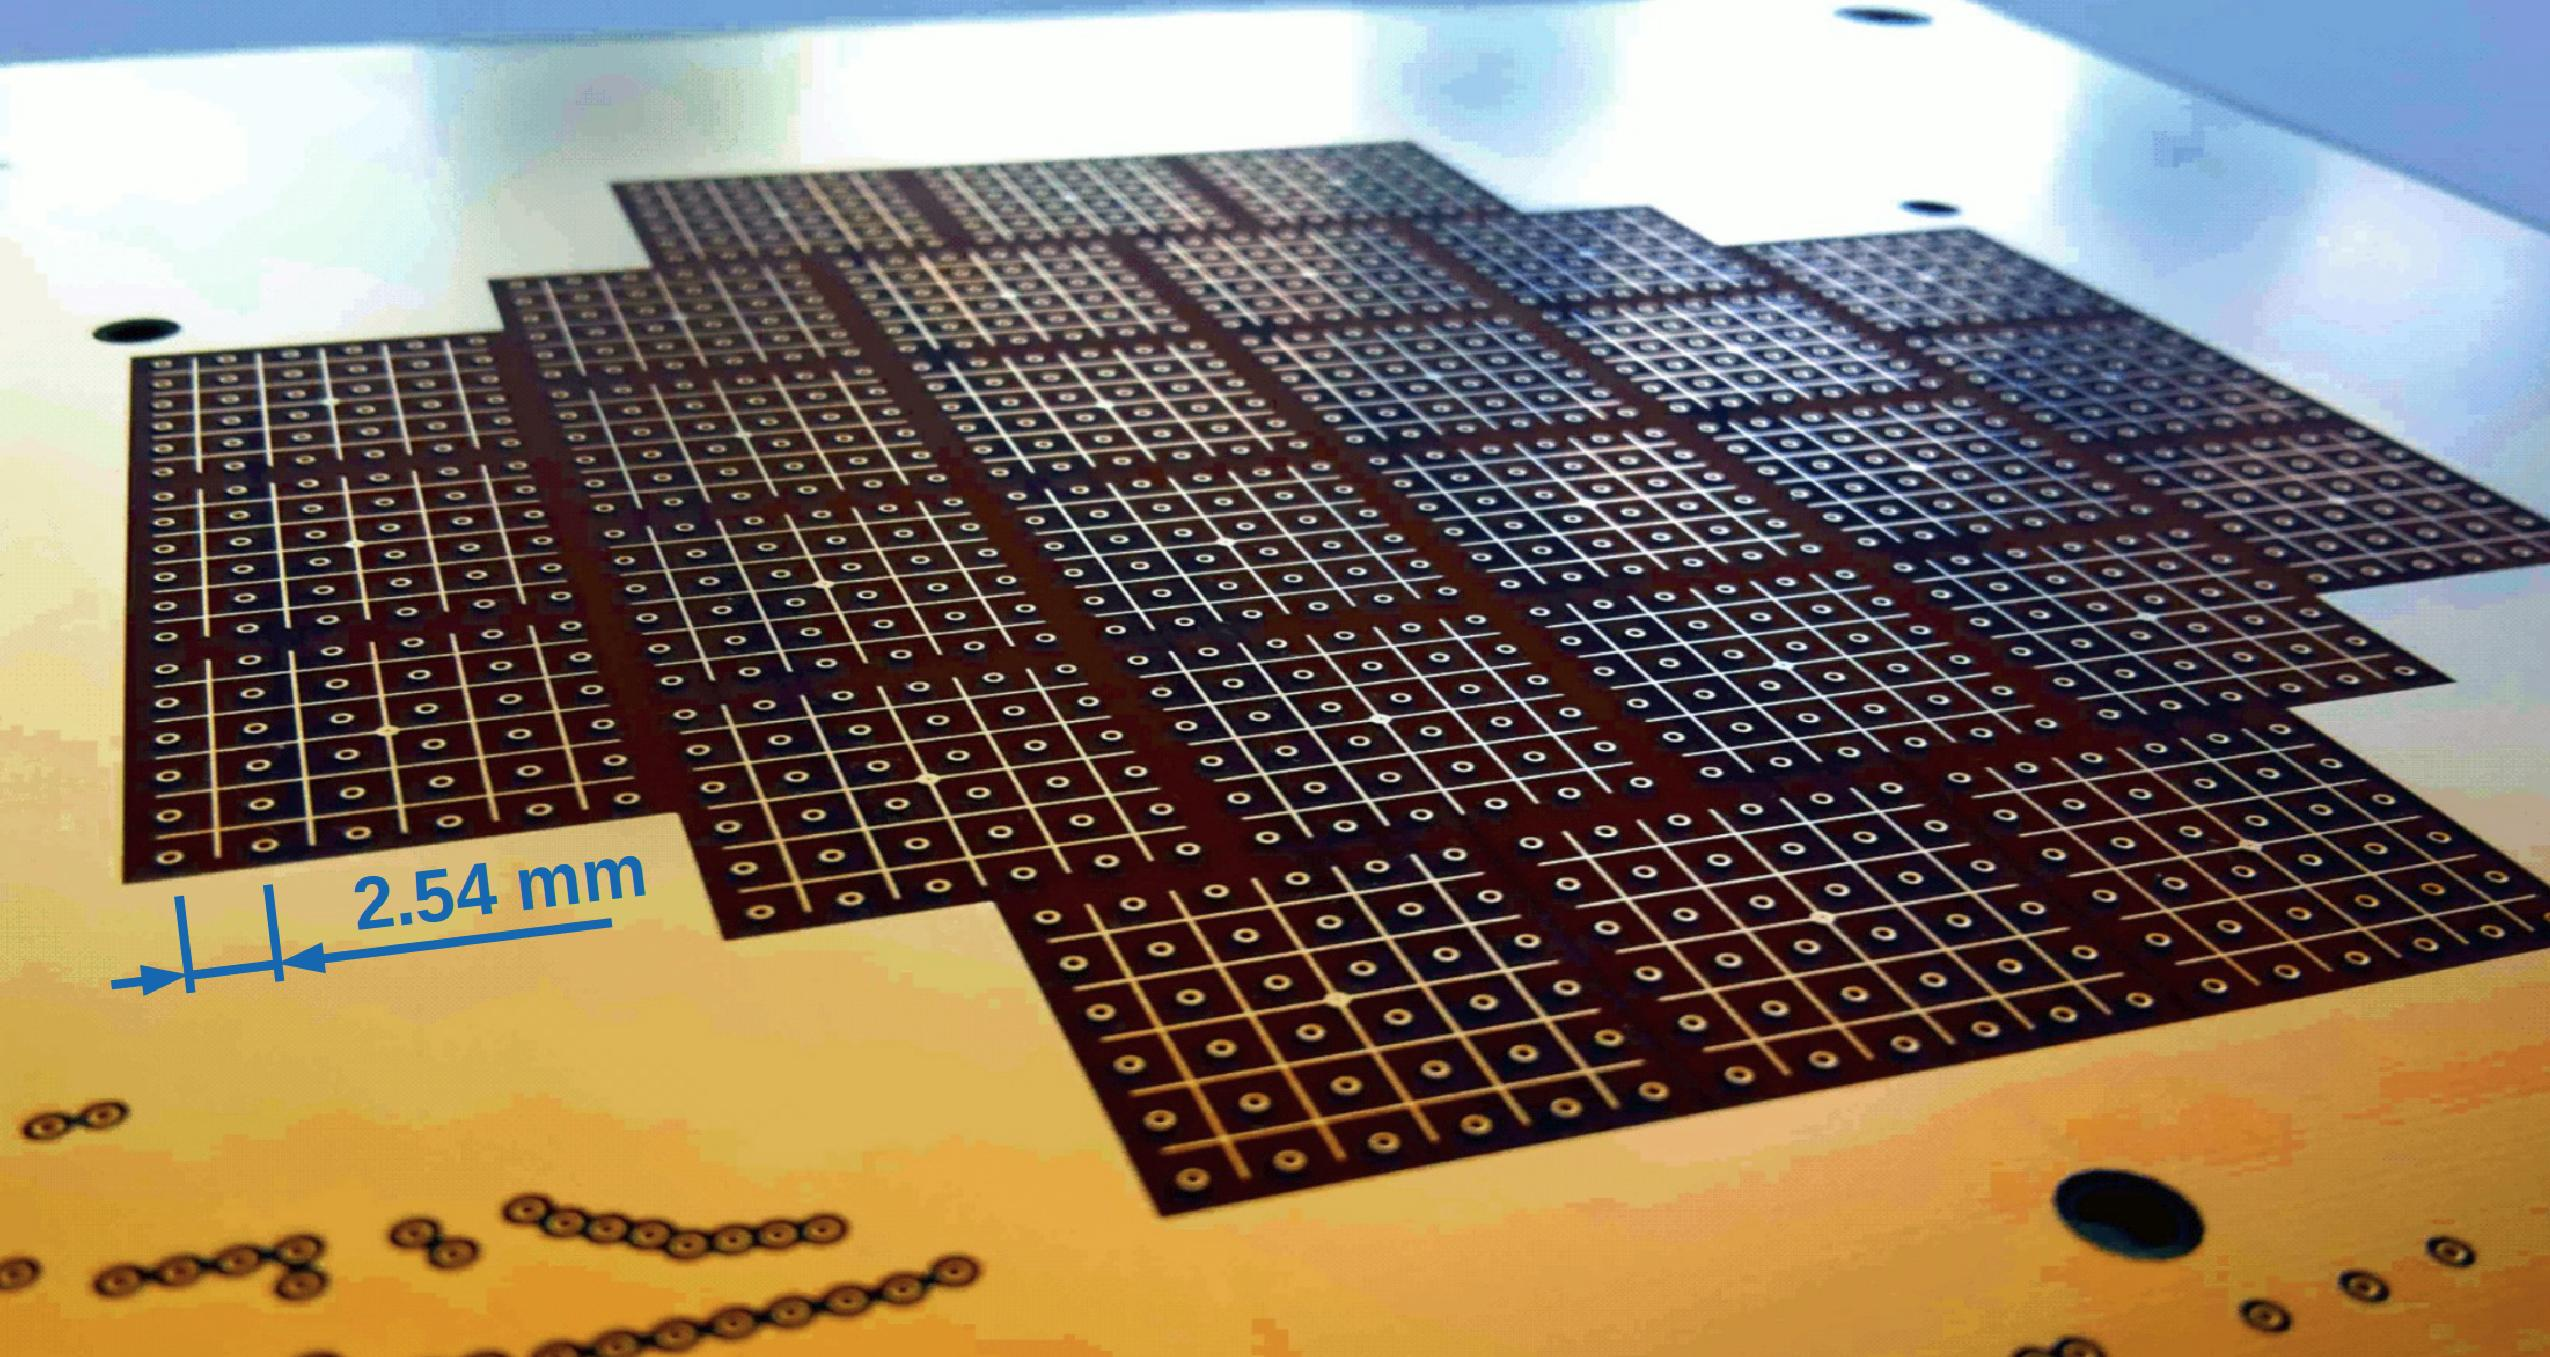
\includegraphics[width=0.65\linewidth]{Figures/pixies.jpg}
	\caption{Initial (July 2016) prototype pixelated anode PCB. The pixelated readout area is \SI{100}{\milli\metre} in diameter.
		Each charge collection pixel is a \SI{900}{\micro\metre} via, at a pitch of \SI{2.54}{\milli\metre}, inductive focusing grids formed of \SI{152.4}{\micro\metre} copper traces surround the pixels. The inductive focusing grid is split into 28 Regions of Interest (ROIs). There are 36 pixels per ROI, a total of 1008 pixels.}
	\label{fig:pixies}
\end{figure}

Vias were used for pixels instead of pads in order to minimise capacitance.
It is important that capacitance is minimised when detecting charge since thermal noise ($Q_{\mathrm{Noise}}$) scales with capacitance ($C$) according to
\begin{equation}
	Q_{\mathrm{Noise}} = \sqrt{k_{\mathrm{B}}TC} \mathrm{,}
\end{equation}
where $k_{\mathrm{B}}$ is the Boltzmann constant, and $T$ the temperature (derived from~\cite{noise}).
It should be noted that the dependence on capacitance can become even stronger depending on the preamplifier used.
However, as we want to keep considerations as general as possible, the influence of the preamplifier will not be discussed here.
To further minimise parasitic capacitance, the PCB design was optimised by removing unnecessary ground planes, routing signal tracks outside necessary ground planes, and increasing the thickness of the PCB to \SI{3.5}{\milli\metre} from an initial \SI{1.75}{\milli\metre}. 
Capacitance at each pixels is $\order{\SI{50}{\pico\farad}}$, however a significant contribution to this is due to additional traces required for the multiplexing scheme.

As shown in Figure~\ref{fig:circuit}, the pixels are directly coupled to the preamplifiers.
The inductive focusing grids are coupled to the preamplifiers via a \SI{10}{\nano\farad} capacitor, and are connected to the bias voltage via a \SI{10}{\mega\ohm} resistor and a low-pass RC filter used to remove AC ripples from the DC bias. 
The RC filter consists of another \SI{10}{\mega\ohm} resistor and a \SI{10}{\nano\farad} capacitor to ground.   

\begin{figure}[htb]
	\centering
	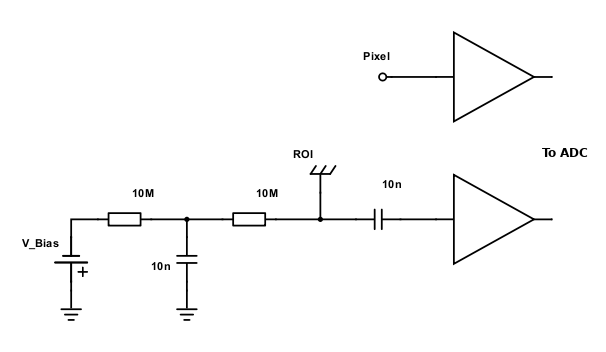
\includegraphics[width=0.65\linewidth]{Figures/schemeit-project_mod}
	\caption{Circuit diagram for pixels and inductive focusing grids that form the Regions Of Interest (ROIs). Pixels are directly coupled to the preamplifiers. ROIs are coupled to the preamplifiers via a \SI{10}{\nano\farad} capacitor, and are connected to the bias voltage via a \SI{10}{\mega\ohm} resistor and a low-pass RC filter used to remove AC ripples from the DC bias. The filter consists of another \SI{10}{\mega\ohm} resistor and a \SI{10}{\nano\farad} capacitor to ground.}
	\label{fig:circuit}
\end{figure}

The bias on the inductive focusing grids had to be sufficient to allow full charge transparency (all charge collected by the pixels), yet low enough to minimise any risk of damaging the cold coupling capacitors.
We took measurements with bias voltages varying from \SIrange{0}{300}{\volt} DC.
Optimal results were achieved at \SI{250}{\volt}.

\subsection{Readout Scheme}

Cryogenic preamplifiers were used to minimise both the noise-sensitive unamplified signal path and the thermal noise introduced by the amplifier itself~\cite{art_cold_ero}.
The preamplifier Application Specific Integrated Circuits (ASICs) used are the LARASIC4*~\cite{larasic} designed by the Brookhaven National Lab, first tested in the ARGONTUBE experiment~\cite{art_cold_ero} and deployed in the MicroBooNE and LArIAT experiments~\cite{uboner,lariat}.
LARASIC4*s were designed for traditional wire readouts, which require fewer channels than a pixelated readout of equivalent dimensions and pitch. 
Therefore, no focus was placed on high channel density, and the LARASIC4*s have only 16 channels per chip.
Given the 1008 pixels, cold digitisation is disfavoured due to power consumption constraints. 
Ideally, every pixel would be read out and the signals then digitally multiplexed, requiring bespoke pixel ASIC capable of cold amplification and digitisation for many channels.
Such ASICs are being developed by Lawrence Berkeley National Lab~\cite{larpix}, as a result of this work. 
Therefore, analogue multiplexing had to be used to minimise the channel numbers, with signals digitised at room temperature outside the cryostat.

\begin{figure}[htb]
	\centering
	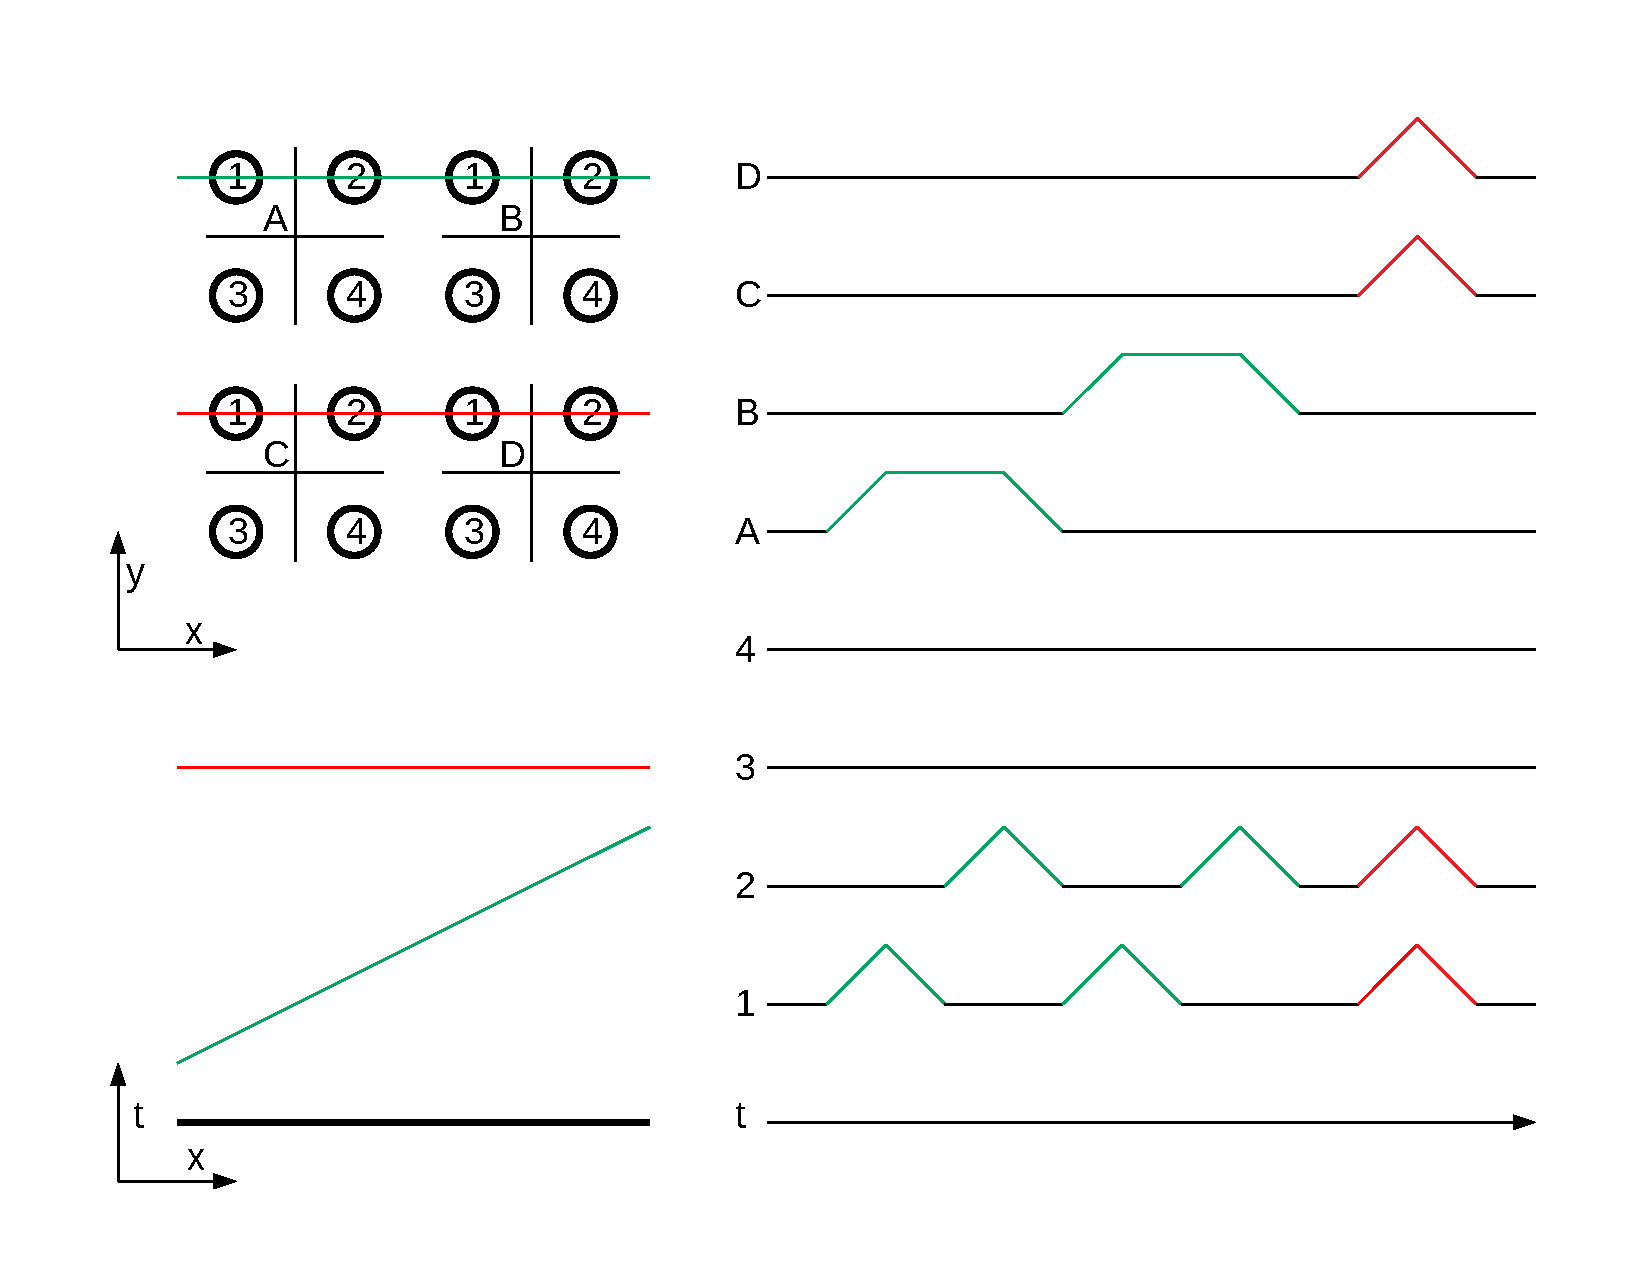
\includegraphics[width=\textwidth]{Figures/mux}
	\caption{Example of the multiplexing scheme: readout plane with ionisation tracks on the left, DAQ waveforms on the right. 16 pixels are read out by 4 DAQ channels (\numrange{1}{4}) by connecting four pixels to each of the four DAQ channels. In addition, four DAQ channels are required to read out the four inductive grids A to D required to derive the physical position of the collecting pixel, regions of interest (ROIs). Dashed green and solid red lines are two examples of ionisation tracks. The green track, inducing a signal in only one grid simultaneously can be reconstructed unambiguously. However, the red track induces signals in grids C and D simultaneously, the physical position of the collecting pixels cannot be unambiguously derived purely from the acquired waveforms. Note that geometry, timing, and pulse shapes are not to scale. Induction signals are, however, unipolar also in reality because the ionisation charge does not drift past the induction grids as in a conventional wire readout.}
	\label{fig:mux}
\end{figure}

As mentioned, the multiplexing scheme divides the pixel plane into a number of ROIs, where each ROI is defined as the pixels contained within a single section of inductive focusing grid. 
The following is taken from Ref~\cite{maplesyrup}.
All pixels at the same coordinate inside each of the ROIs are connected to the same DAQ channel, i.e. only one DAQ channel connects all the pixels in the top left corners of all ROIs, and so on.
A simple example is shown in Figure~\ref{fig:mux}, which demonstrates how 16 physical pixels can be read out using only 8 DAQ channels. 
For an optimal expression of the multiplexing scheme, a pixel plane of $N \times N$ pixels (where $N = n ^ 2$ and $n$ integer) is divided into $n \times n$~ROIs, each ROI containing, again, $n \times n = N$ pixels.
Reading out such a plane requires $N$ DAQ channels for the ROIs plus another $N$ channels for the pixels.
With the employed multiplexing scheme, only as many pixel channels as there are pixels per ROI are required, due to the fact that all pixels at the same relative position across all ROIs share a common DAQ channel.
This means that an $N \times N$ pixel plane requires only $2 N$ DAQ channels; the same as a conventional 2-plane wire readout of the same pitch, and dimension.
Optimising the number of ROIs allowed us to readout the 1008 physical pixels with only 64 DAQ channels (28 ROIs + 36 pixels).
The non-square numbers are the result of geometrical constraints on our readout plane.

Pixel signals are then associated to an induction signal on the ROI grid as follows. 
If there is a signal on a certain pixel DAQ channel, the position inside the ROI is known, but not which ROI the hit occurred in.
By combining the inductive bipolar pulse on the ROI grid with any simultaneous collection pulses from the pixels, it is possible to disentangle the true position.
Again, the drawback of this approach is that it is not free from ambiguities; it fails for multiple simultaneous hits when it is impossible to say which pixel pulse belongs to which ROI pulse.
Ambiguous hits are flagged as pixel signals corresponding to multiple ROI signals, which can be disentangled later using reconstruction tools. 

\subsection{Pixel Demonstration TPC} \label{sec:viper}

The pixel demonstration TPC, shown in Figures~\ref{fig:schematic}~and~\ref{fig:v1per}, is cylindrical with an inner diameter of \SI{101}{\milli\metre} and a \SI{590}{\milli\metre} drift length. 
The TPC operated with a drift field of \SI{1}{\kilo\volt\per\centi\metre}, corresponding to a total drift time of \SI{281}{\micro\second}. 
The field-cage consists of aluminium rings supported by clear acrylic rings, with a cathode formed of a brass disc. 
The dimensions of the field-cage and cathode are shown in Figure~\ref{fig:schematic}.
Alternating acrylic rings are split, to allow for the circulation of purified LAr within the TPC volume, there are twenty complete rings.
Four square section PAI\footnote{Polyamide-imide} uprights support the cathode and field cage, with PEEK\footnote{Polyether ether ketone} screws fixing the pillars to the acrylic rings.
The four PAI uprights connect to a PAI frame which supports the anode plane and a set of  Silicon PhotoMultipliers (SiPMs) for light readout, see Figure~\ref{fig:v1per}. 

\begin{figure}[!ht]
	\centering
	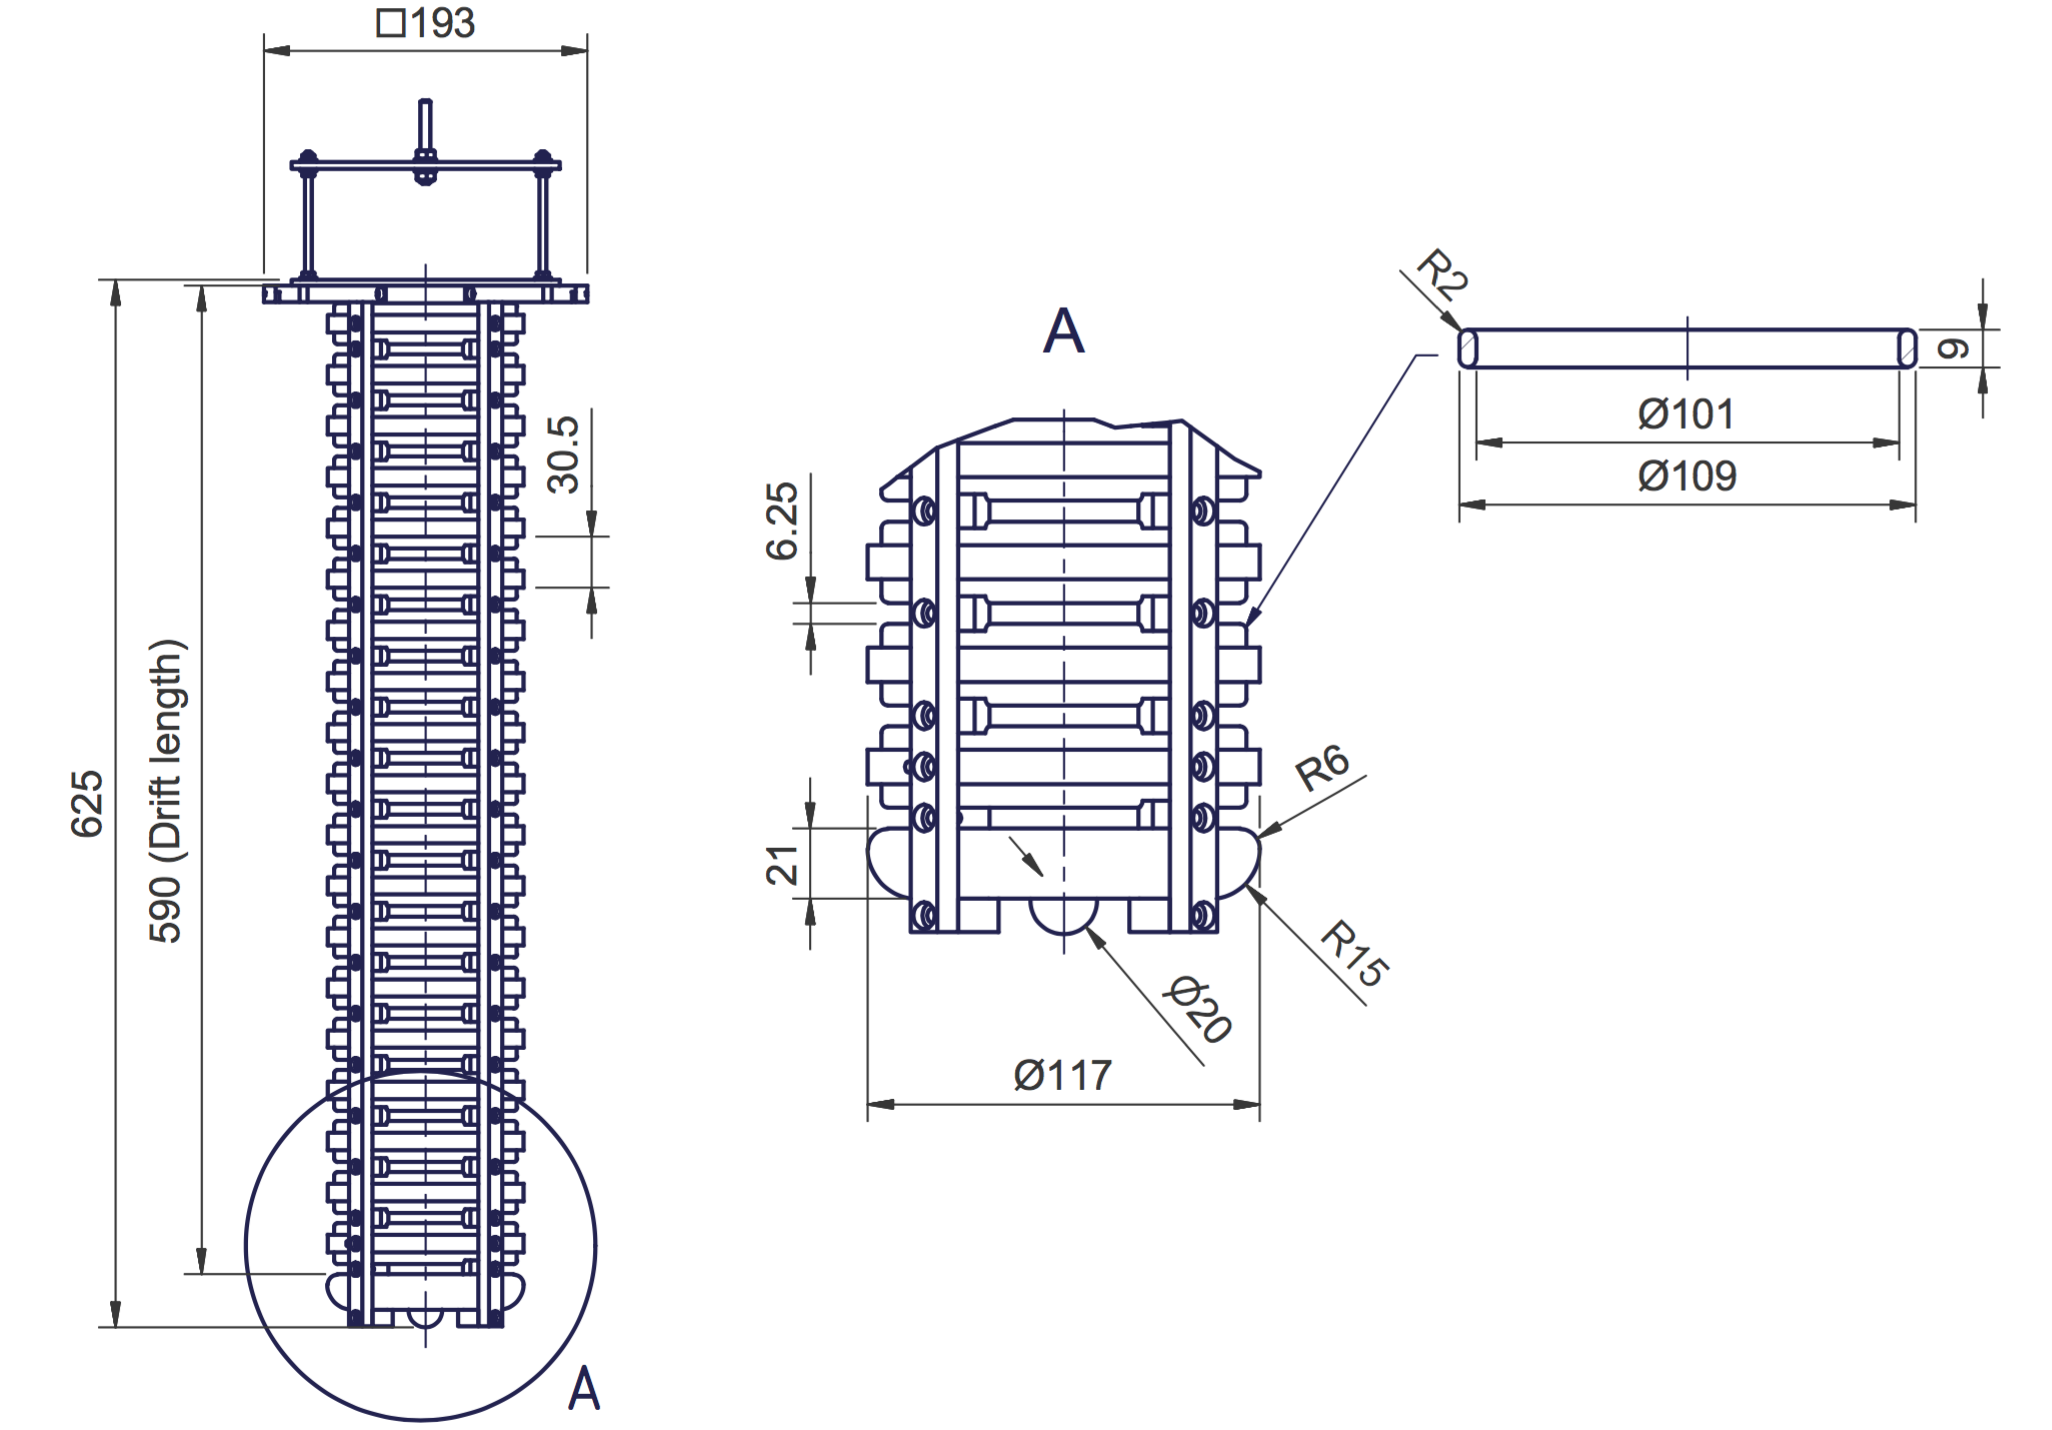
\includegraphics[width=0.9\linewidth]{Figures/Schematic.png}
	\caption{\small Engineering drawing of the pixel demonstration TPC; \SI{590}{\milli\metre} drift length; \SI{6.25}{\milli\metre} field cage spacing; \SI{101}{\milli\metre} internal diameter.}
	\label{fig:schematic}
\end{figure}

The resistive divider consists of a chain of \SI{100}{\mega\ohm} Vishay Rox metal oxide resistors\footnote{ROX100100MFKEL}. Each resistor is soldered to its neighbour, and fixed to the field cage at each joint with an M3 screw.   

\begin{figure}[!ht]
	\centering
	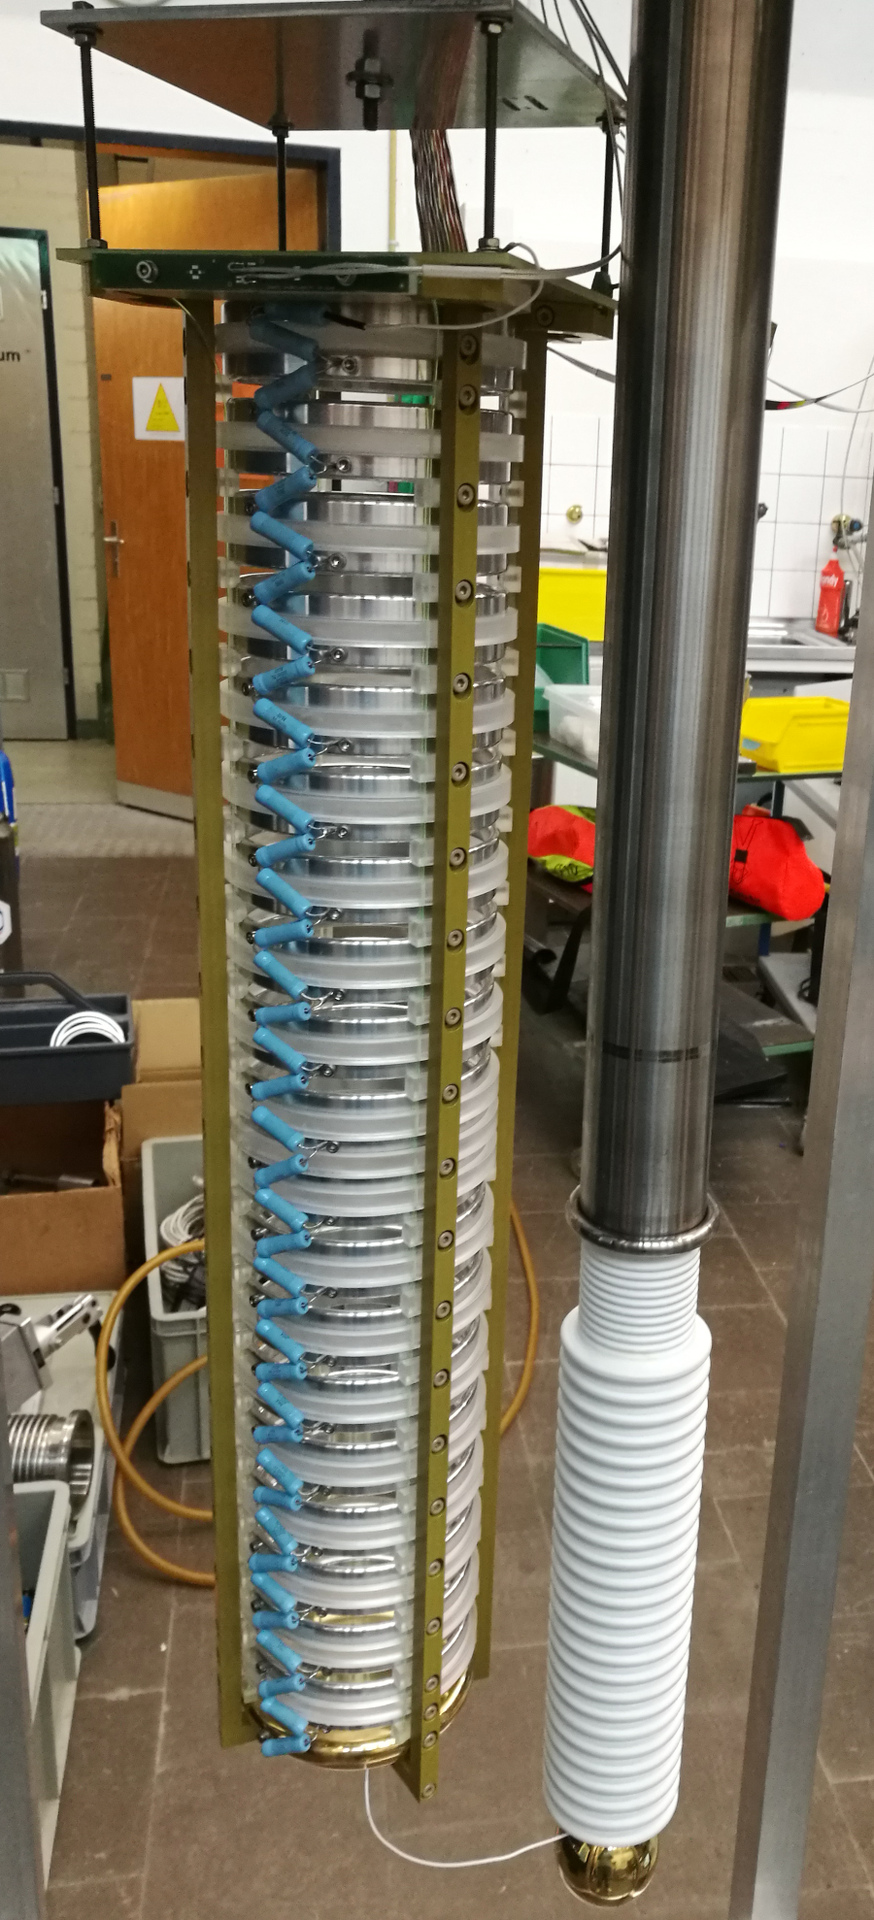
\includegraphics[width=0.26\linewidth]{Figures/viper_original-.jpg}
	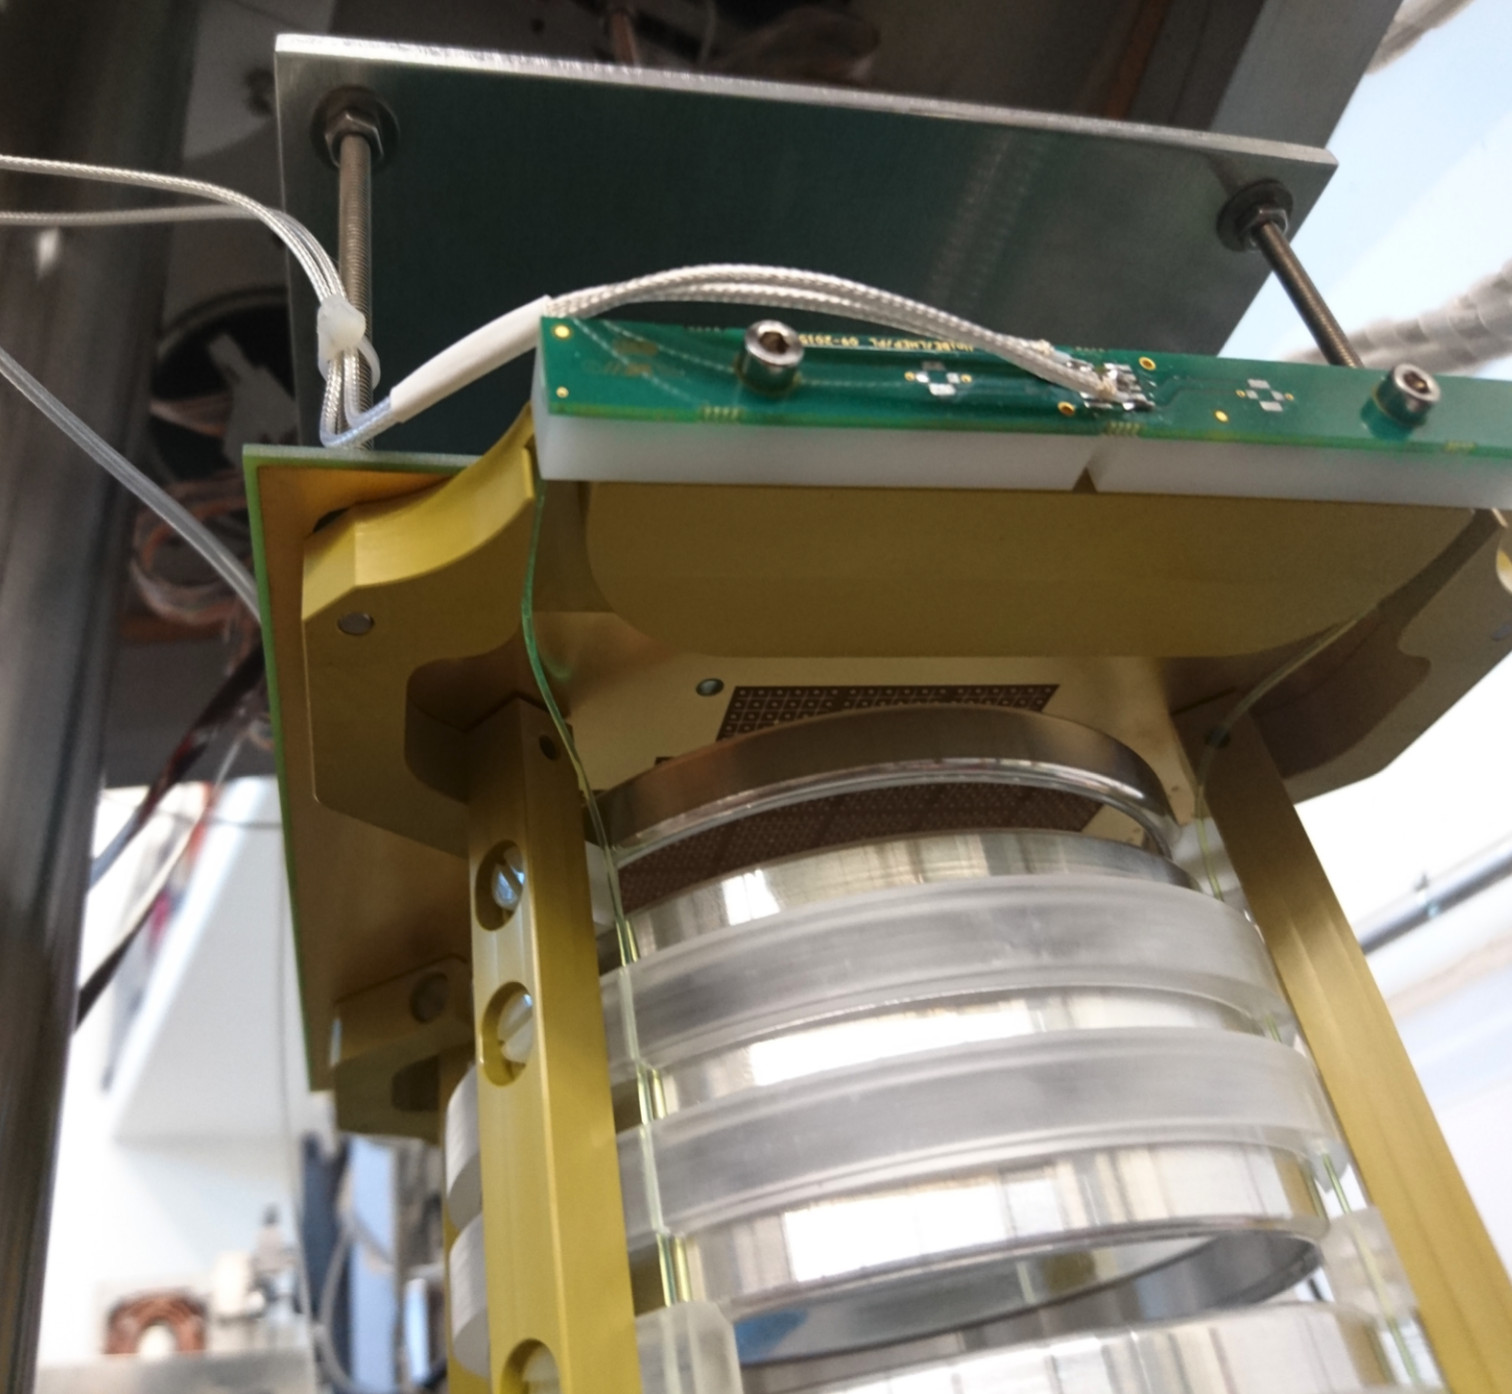
\includegraphics[width=0.62\linewidth]{Figures/viper_sipm-.jpg}
	\caption{\small  Photographs of the  pixel demonstration TPC at Bern, with the HV feedthrough. A close-up of the light collection system shows wavelength shifting fibres coupling SiPMs to the TPB-coated light guides.}
	\label{fig:v1per}
\end{figure}

The acrylic rings provide the light collection; their inner surfaces are machine-polished and coated with the WaveLength Shifter (WLS) TetraPhenylButadiene (TPB). 
The coating method is based on~\cite{TPBcoating}.
\SI{0.5}{\gram} of TPB and \SI{0.5}{\gram} of acrylic flakes were dissolved in \SI{50}{\milli\liter} of toluene and then mixed with \SI{12}{\milli\liter} of ethanol, which serves to increase the coating homogeneity. 
Three layers of the coating were applied by hand, with a fine brush. 

Four WLS fibres of \SI{1}{\milli\metre} diameter (Kuraray Y11(200)M) run vertically next to the PAI uprights, these fibres couple the acrylic rings to four SiPMs (Hamamatsu S12825-050P) mounted close to the anode, see Figure~\ref{fig:v1per}. 
The SiPMs and their front-end electronics were adapted from those developed at Bern for the cosmic ray taggers used in the MicroBooNE and SBND experiments~\cite{CRT, CRT2}.
For operation at LAr temperatures, the SiPM bias voltages had to be reduced from a nominal \SI{70}{\volt} at room temperature to \SI{53}{\volt}, in order to following the drop in breakdown voltage due to temperature.   
In the front-end electronics, two coincidences of two out of the four SiPMs are formed and combined by means of a logic \textit{OR} operation. 
This coincidence is used in order to improve trigger purity.

\subsection{Infrastructure}

The pixel demonstration TPC is housed in a double-bath vacuum-insulated cryostat with the outer bath open to atmosphere for cooling.
The inner LAr is filtered first on filling through a pair of Oxysorb-Hydrosorb filters, and then recirculated through a single custom-made filter containing both activated copper and silica gel.
The cryostat and filtering method were previously used for LAr purity measurements~\cite{purititty}, and High-Voltage (HV) breakdown studies~\cite{HVoriginal}.
Based on these previous studies, an impurity concentration $\order{\SI{1}{ppb}}$ of oxygen-equivalent is estimated, which corresponds to a charge lifetime of \SI{290}{\micro\second}.

The HV feedthrough remains unchanged from the breakdown studies; based on a PET-C polymer dielectric capable of withstanding potentials as high as \SI{-130}{\kilo\volt}.
A low-pass filter was added between the power supply and feedthrough, which consists of an \SI{800}{\pico\farad} decoupling capacitor grounded between two \SI{100}{\mega\ohm} resistors connected in series, all of which is submerged in transformer oil.  

Only the warm signal path of the Data Acquisition (DAQ) was altered from that described in~\cite{protoLASER}, to include differential signalling.
An inverted waveform of the signal is put onto an additional conductor, and the difference is then taken between the signals on the two conductors.
Ground loops are avoided because the signal sink does not need connecting to the same ground as the signal source.
Additionally, the completely symmetric signal path means inductive noise pick-up is equal on both conductors and therefore cancelled at the signal sink.

\section{Data Analysis and Reconstruction} \label{sec:results}

The primary purpose of this experimental set-up is to demonstrate the principle of 3D reconstruction utilising a pixelated charge readout within a LArTPC. 
In this section we focus on both the characterization of the signal to noise ratio and the basic 3D track reconstruction that is made directly possible by this technology.

For reconstruction, the HV for the TPC was set to \SI{-63}{\kilo\volt}, which, after a voltage drop across the HV filter and resistors, corresponds to a \SI{1}{\kilo\volt\per\centi\meter} drift field. The inductive focusing grid was set to a bias of \SI{-300}{\volt}, at which transparency was observed. 

Both drift field and focusing bias were switched off for the noise measurement since the purpose is to characterise only the pixel readout, and not the whole TPC.


\subsection{Signal to noise ratio}

To assess the Signal to Noise Ratio (SNR), dedicated noise data was taken employing a \SI{5}{\hertz} random trigger.
For the \num{2000} recorded events, all pixel and ROI channels were combined respectively and filled into amplitude distribution histograms.
The standard deviation of the two noise distributions was then extracted from a Gauss fit.
This value was used to calculate the noise for pixel and ROI channels according to
\begin{equation}
\m{SNR} = \frac{S}{\sigma}\,\m{,}
\label{eq:snr}
\end{equation}
where $\sigma$ is the noise standard deviation from the Gaussian fit and $S$ is the expected signal, which will be explained in detail below.
As can be seen in Figure~\ref{fig:unfilteredRawData_a}, pixel channel number~\num{10} is significantly noisier in comparison to others, likely caused by a broken preamplifier.
Therefore, this channel was blinded for the SNR calculations.
The resulting equivalent noise charge is \SI{1095}{\elementarycharge} for the pixel channels and \SI{982}{\elementarycharge} for the inductive ROI channels.

The signal $S$ is often taken for a Minimum-Ionising Particle (MIP) as this is a typical low-amplitude signal interesting for neutrino physics.
Correctly deriving the deposited charge from experimental data requires a calibrated event reconstruction which was not available at the time of writing.
Therefore, we estimated the MIP signal from theory assuming an energy loss of \SI{2.1}{\mega\electronvolt\per\centi\metre}~\cite{pdg}.
This can be converted to charge loss using the energy required to produce one electron-ion pair: $W_{\m{i}} = \SI{23.6}{\electronvolt\per\elementarycharge}$~\cite{NobleGasDetectors}.
Additionally, charge recombination, diffusion and attachment losses characterised by lifetime need to be taken into account.
The recombination factor was measured by both ICARUS and ArgoNeuT~\cite{icarusReco, argoneutReco}, and found to be $R_{\m{c}} \approx 0.7$ for a drift field of $\SI{1}{\kilo\volt\per\centi\meter}$.
For a non-zero drift field, diffusion needs to be split into longitudinal and transverse components.
Using the ARGONTUBE detector~\cite{argontube}, we earlier measured a transverse diffusion coefficient of $D_{\m{T}} = \SI{5.3}{\centi\metre\squared\per\second}$ at \SI{0.25}{\kilo\volt\per\centi\metre} while Gushchin et al.~\cite{gushchin} report a value of $D_{\m{T}} = \SI{13}{\centi\metre\squared\per\second}$ at \SI{1}{\kilo\volt\per\centi\metre}.
Even using the more conservative value, this results~\cite{lngDet} in a transverse spread of
\begin{equation}
\sigma_{\m{T}} = \sqrt{2 D_{\m{T}} t} \approx \SI{0.9}{\milli\metre}\,, 
\end{equation}
for our drift time of $t = \SI{281}{\micro\second}$; a value well below the pixel pitch of $d_{\m{p}} = \SI{2.54}{\milli\metre}$.
Considering that the longitudinal component is smaller than the transverse ~\cite{lngDet}, we neglect diffusion completely for our calculations.
Finally, our lifetime of \SI{290}{\micro\second} reduces the charge to $\approx\SI{38}{\percent}$ over the full drift distance.
Combining this, we get a signal of 
\begin{equation}
S = \dv{E}{x}_{\m{MIP}} \frac{R_{\m{c}} d_{\m{p}}}{W_{\m{i}}} = \SI{15821}{\elementarycharge}\,,
\end{equation}
for a charge deposited adjacent to the readout plane, and $S = \SI{6004}{\elementarycharge}$ for a charge deposited adjacent to the cathode.

Table~\ref{tab:snr} lists the SNR values obtained from these signal values and the aforementioned measured equivalent noise charge, using Equation~\eqref{eq:snr}.

\begin{table}[htb]
	\centering
	\caption{SNR values obtained from Equation~\eqref{eq:snr} using the theoretical signal of a MIP at the readout plane or cathode, respectively combined with the average equivalent noise charge for pixel and ROI channels obtained from measurements.}
	\label{tab:snr}
	\begin{tabu} to \textwidth {|l|l|S|}
		\hline
		{Channel} &	{MIP at} &			{SNR} \\
		\hline
		\hline
		{Pixel} &	{Readout plane} &	\num{14} \\
		\hline
		{Pixel} &	{Cathode} &			\num{5.5} \\
		\hline
		{ROI} &		{Readout plane} &	\num{16} \\
		\hline
		{ROI} &		{Cathode} &			\num{6.1} \\
		\hline
	\end{tabu}
\end{table}

\clearpage 

\subsection{3D track reconstruction}

A sample of several thousand cosmic ray events were collected, mostly minimum ionising muons traversing the TPC, to demonstrate 3D track reconstruction.
These events were triggered by the light readout described in Section~\ref{sec:viper}.

The reconstruction procedure comprises five steps:
\begin{enumerate}
	\item Noise filtering
	\item Pulse finding
	\item 3D hit finding
	\item Ambiguity rejection
	\item Track fitting
\end{enumerate}

These steps are explained in the following and depicted in Figures~\ref{fig:unfilteredRawData} through~\ref{fig:kalman}, all taken from the same MIP (cosmic muon) event.

In the first step, a noise-filtering algorithm is applied to the raw data.
As can be seen from Figure~\ref{fig:unfilteredRawData}, the noise is largely correlated across all the channels\footnote{Due to the much higher signal levels, the noise is barely visible on the pixel channels in Figure~\ref{fig:unfilteredRawData_a}.}.
This common-mode correlation can be exploited by the noise filter algorithm.
The following is done separately for the all pixel and ROI channels of each event.
Similarly to the SNR calculation, all samples are filled into an amplitude distribution histogram for each channel, and subsequently fitted with a Gaussian distribution.
A noise band is defined per channel with its centre equal to the mean of the Gauss fit and its width equal to the standard deviation multiplied by a tunable scaling factor.
The signal amplitudes of all channels within the corresponding noise band are then averaged for each sample.
Finally, this average is subtracted from each channel at the corresponding sample.
We chose this technique because it effectively suppresses the dominating common mode noise.
At the same time, spurious signals produced by high amplitudes from collected charge distorting the average are kept to a minimum by only accepting values within the noise band.
The effectiveness of the filtering can be seen in Figure~\ref{fig:filteredRawData}, showing the same raw data as Figure~\ref{fig:unfilteredRawData} post filtering.

\begin{figure}[htb]
	\centering
	\begin{subfigure}{\textwidth}
		\centering
		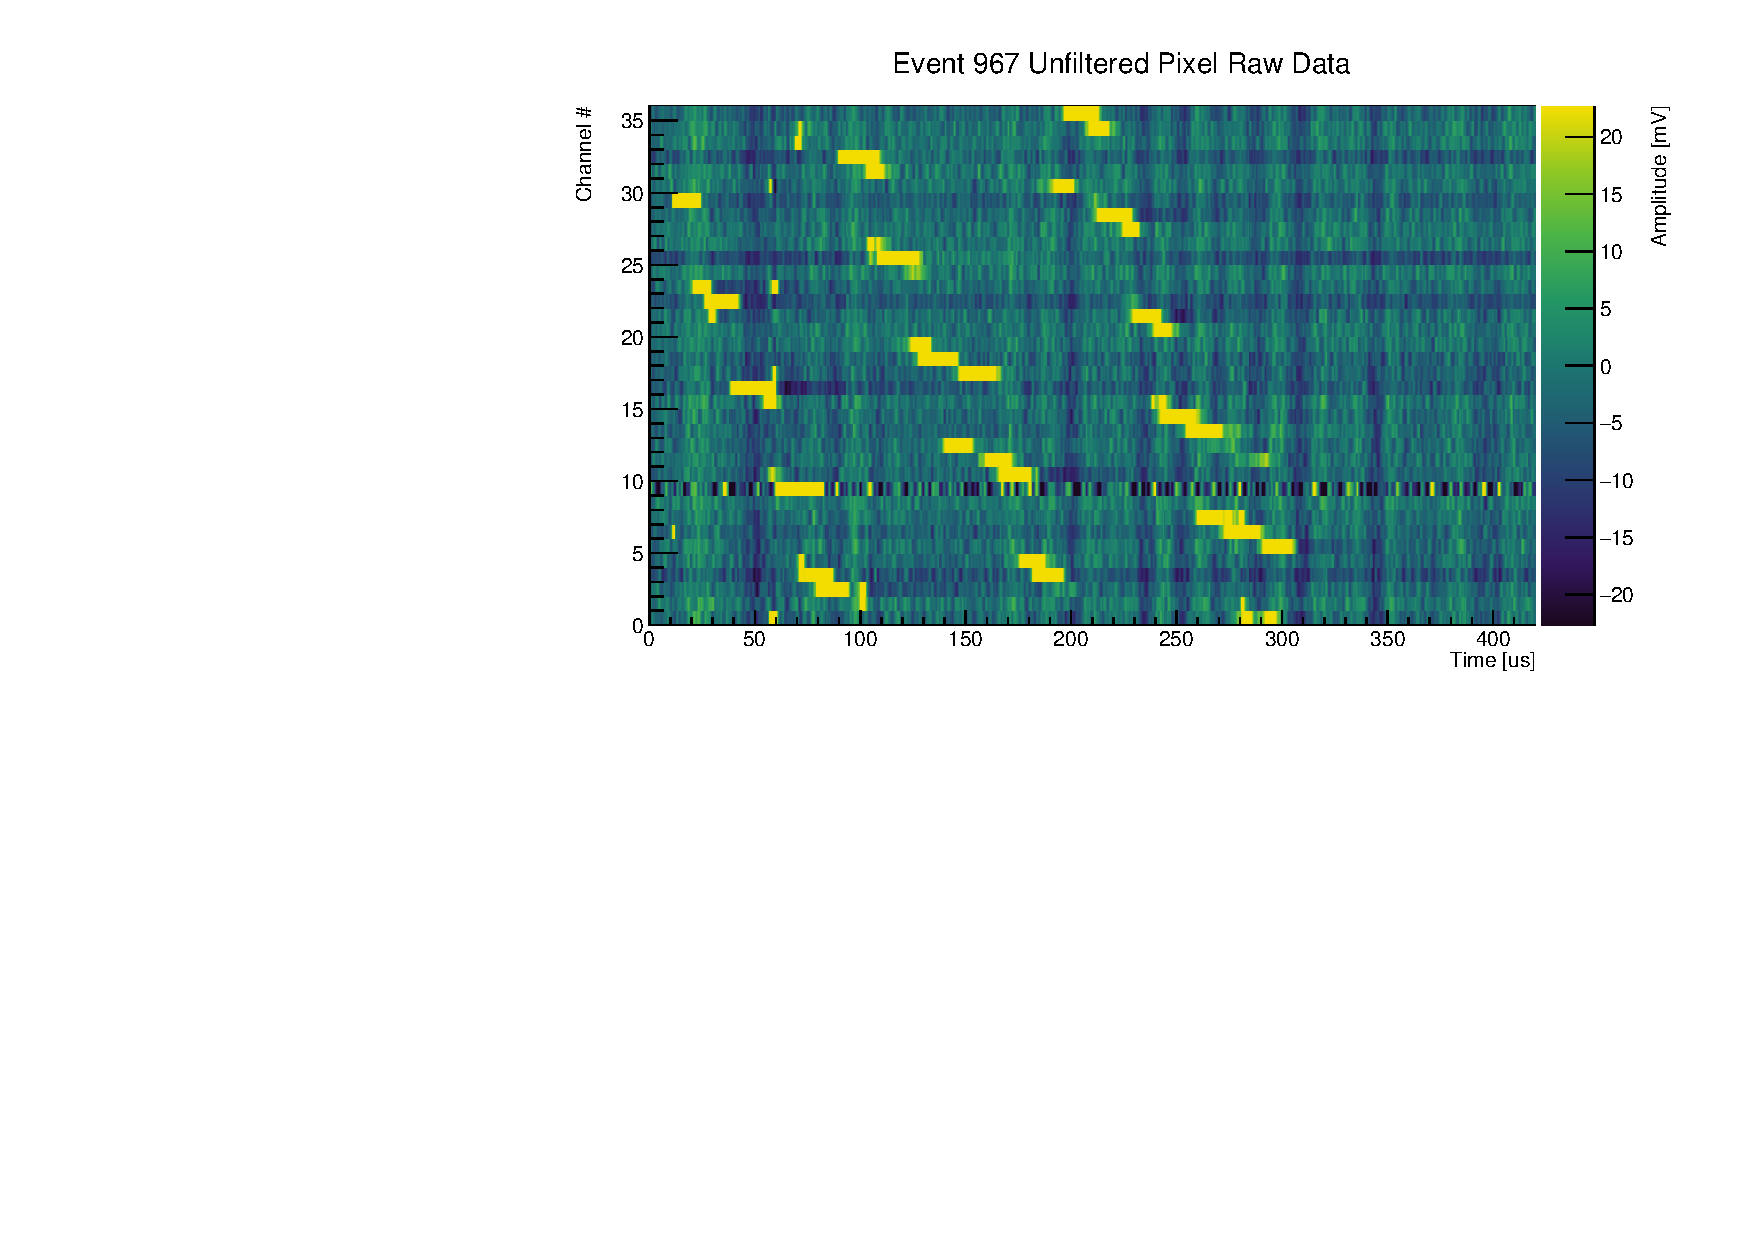
\includegraphics[viewport=0 0 550 290, clip, width=\textwidth]{event967_rawUnfilteredPixel}
		\caption{Pixel raw data\\.}
		\label{fig:unfilteredRawData_a}
	\end{subfigure}
	\begin{subfigure}{\textwidth}
		\centering
		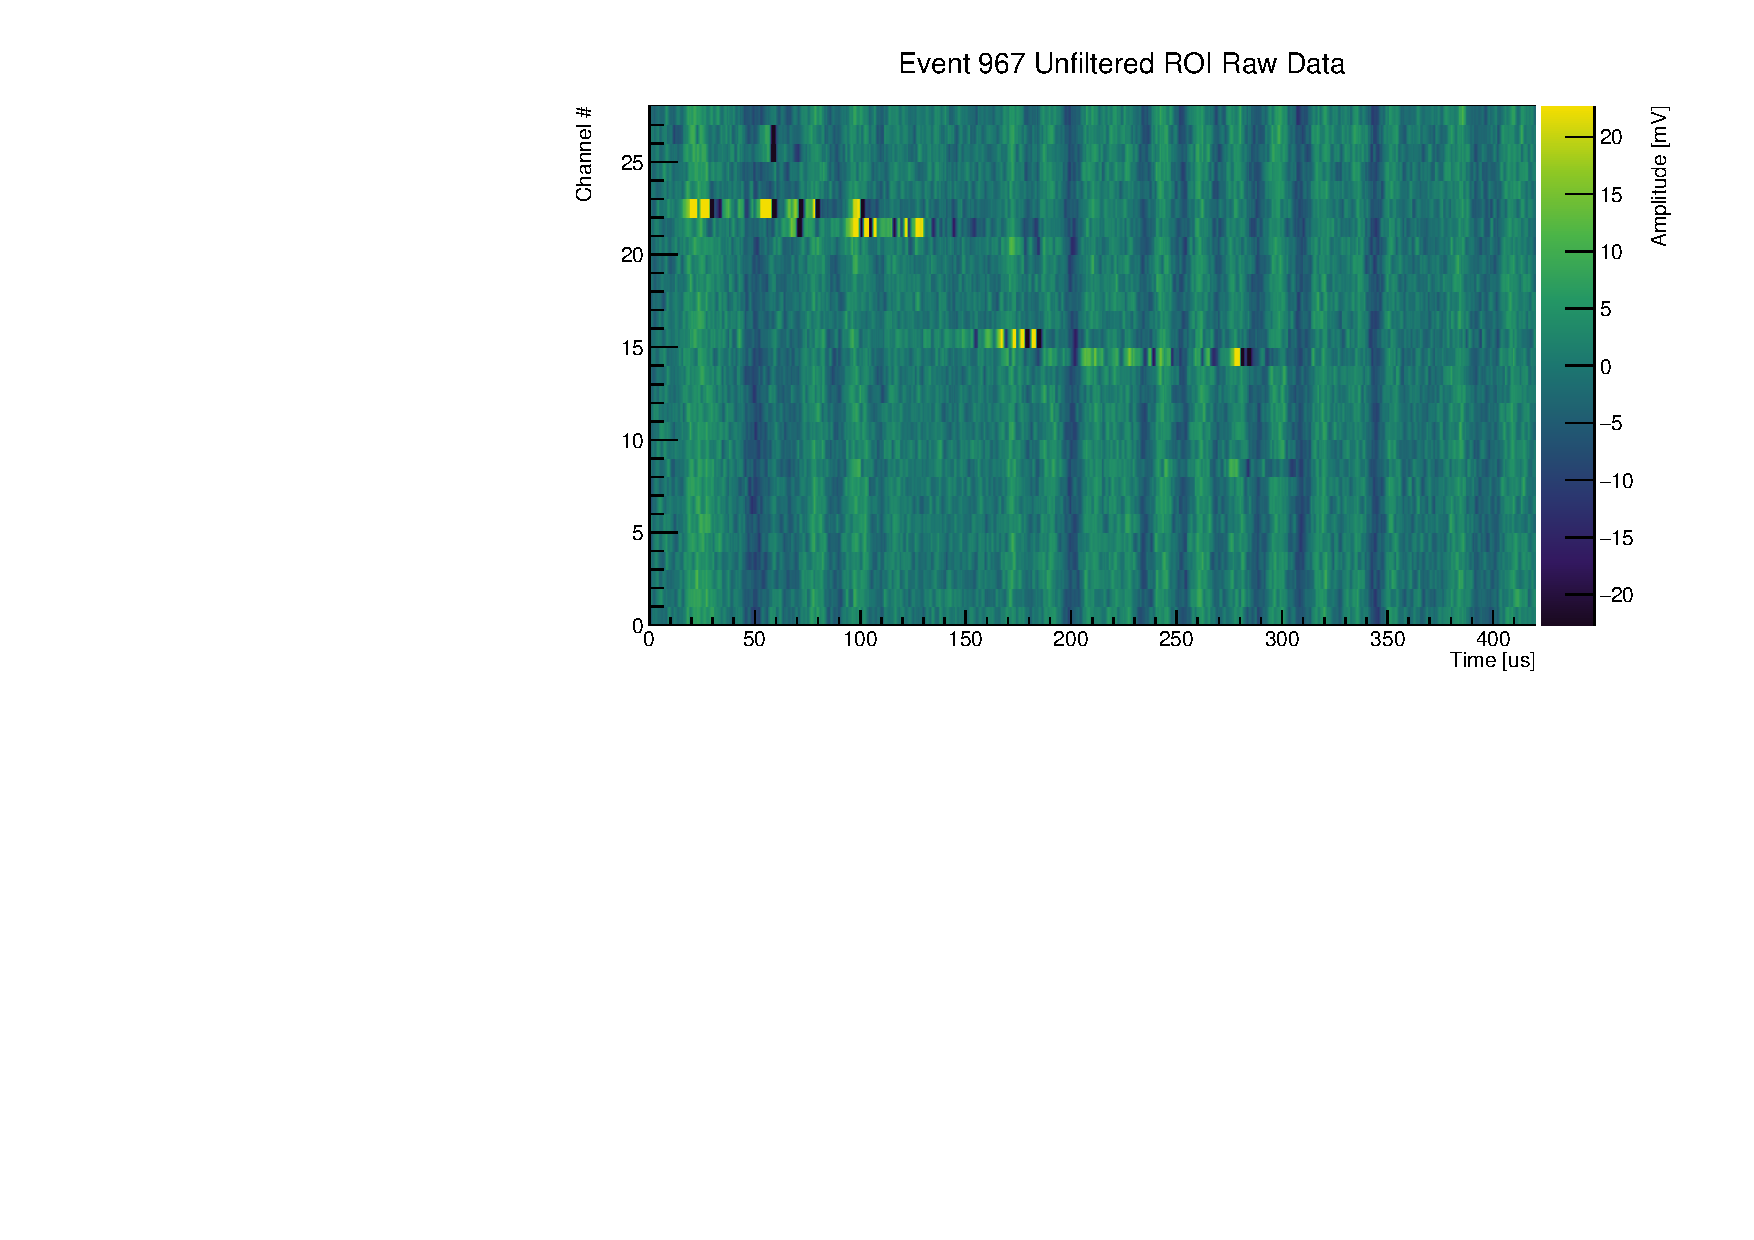
\includegraphics[viewport=0 0 550 290, clip, width=\textwidth]{event967_rawUnfilteredROI}
		\caption{ROI raw data}
		\label{fig:unfilteredRawData_b}
	\end{subfigure}
	\caption{Unfiltered raw data of a typical MIP event (the same event as in Figures~\ref{fig:filteredRawData} through~\ref{fig:kalman}).
		Note that the colour scale was adjusted to highlight the charge signals.
		Therefore, most signal peaks are above/below the maximum/minimum of the colour scale.
		The full range of a typical signal can be seen in Figure~\ref{fig:hitFinder}.}
	\label{fig:unfilteredRawData}
\end{figure}

\begin{figure}[htb]
	\centering
	\begin{subfigure}{\textwidth}
		\centering
		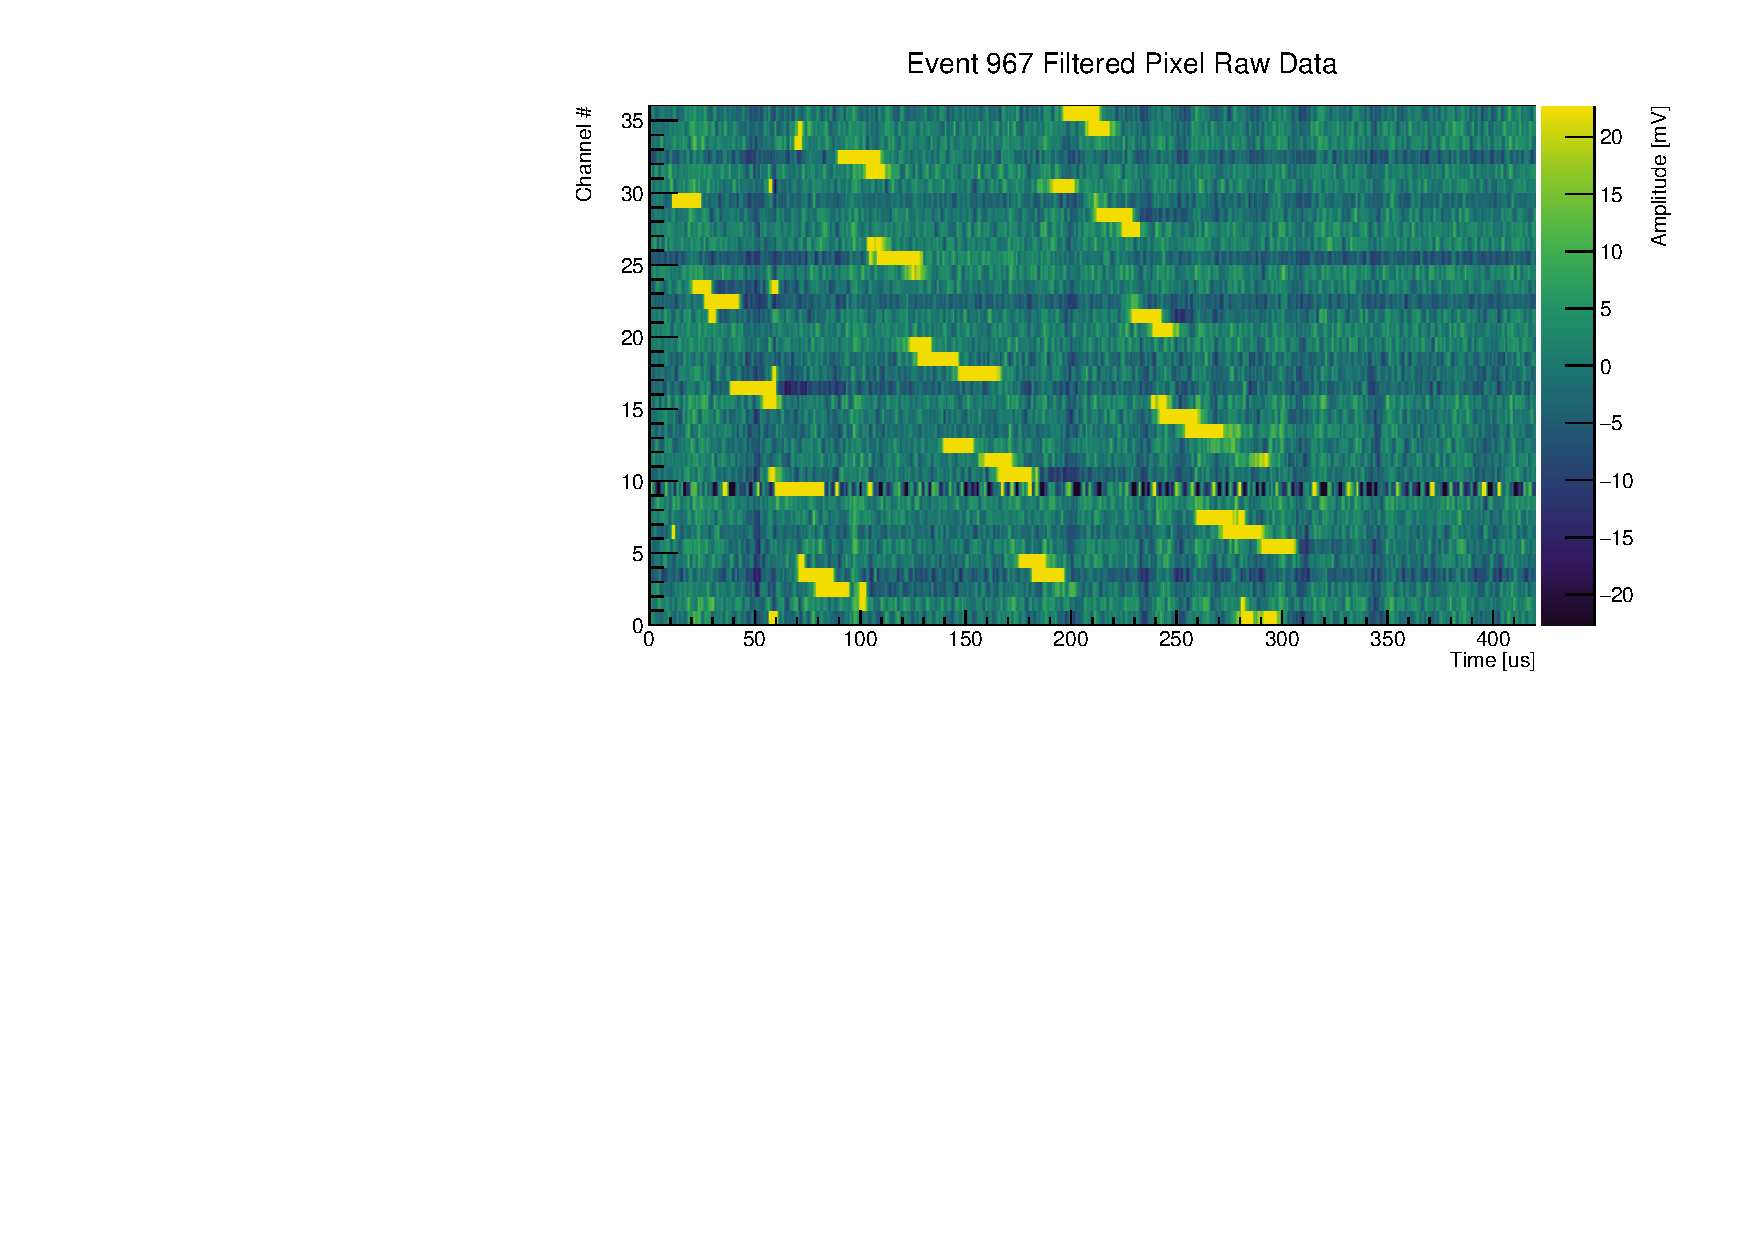
\includegraphics[viewport=0 0 550 290, clip, width=\textwidth]{event967_rawFilteredPixel}
		\caption{Pixel raw data\\.}
		\label{fig:filteredRawData_a}
	\end{subfigure}
	\begin{subfigure}{\textwidth}
		\centering
		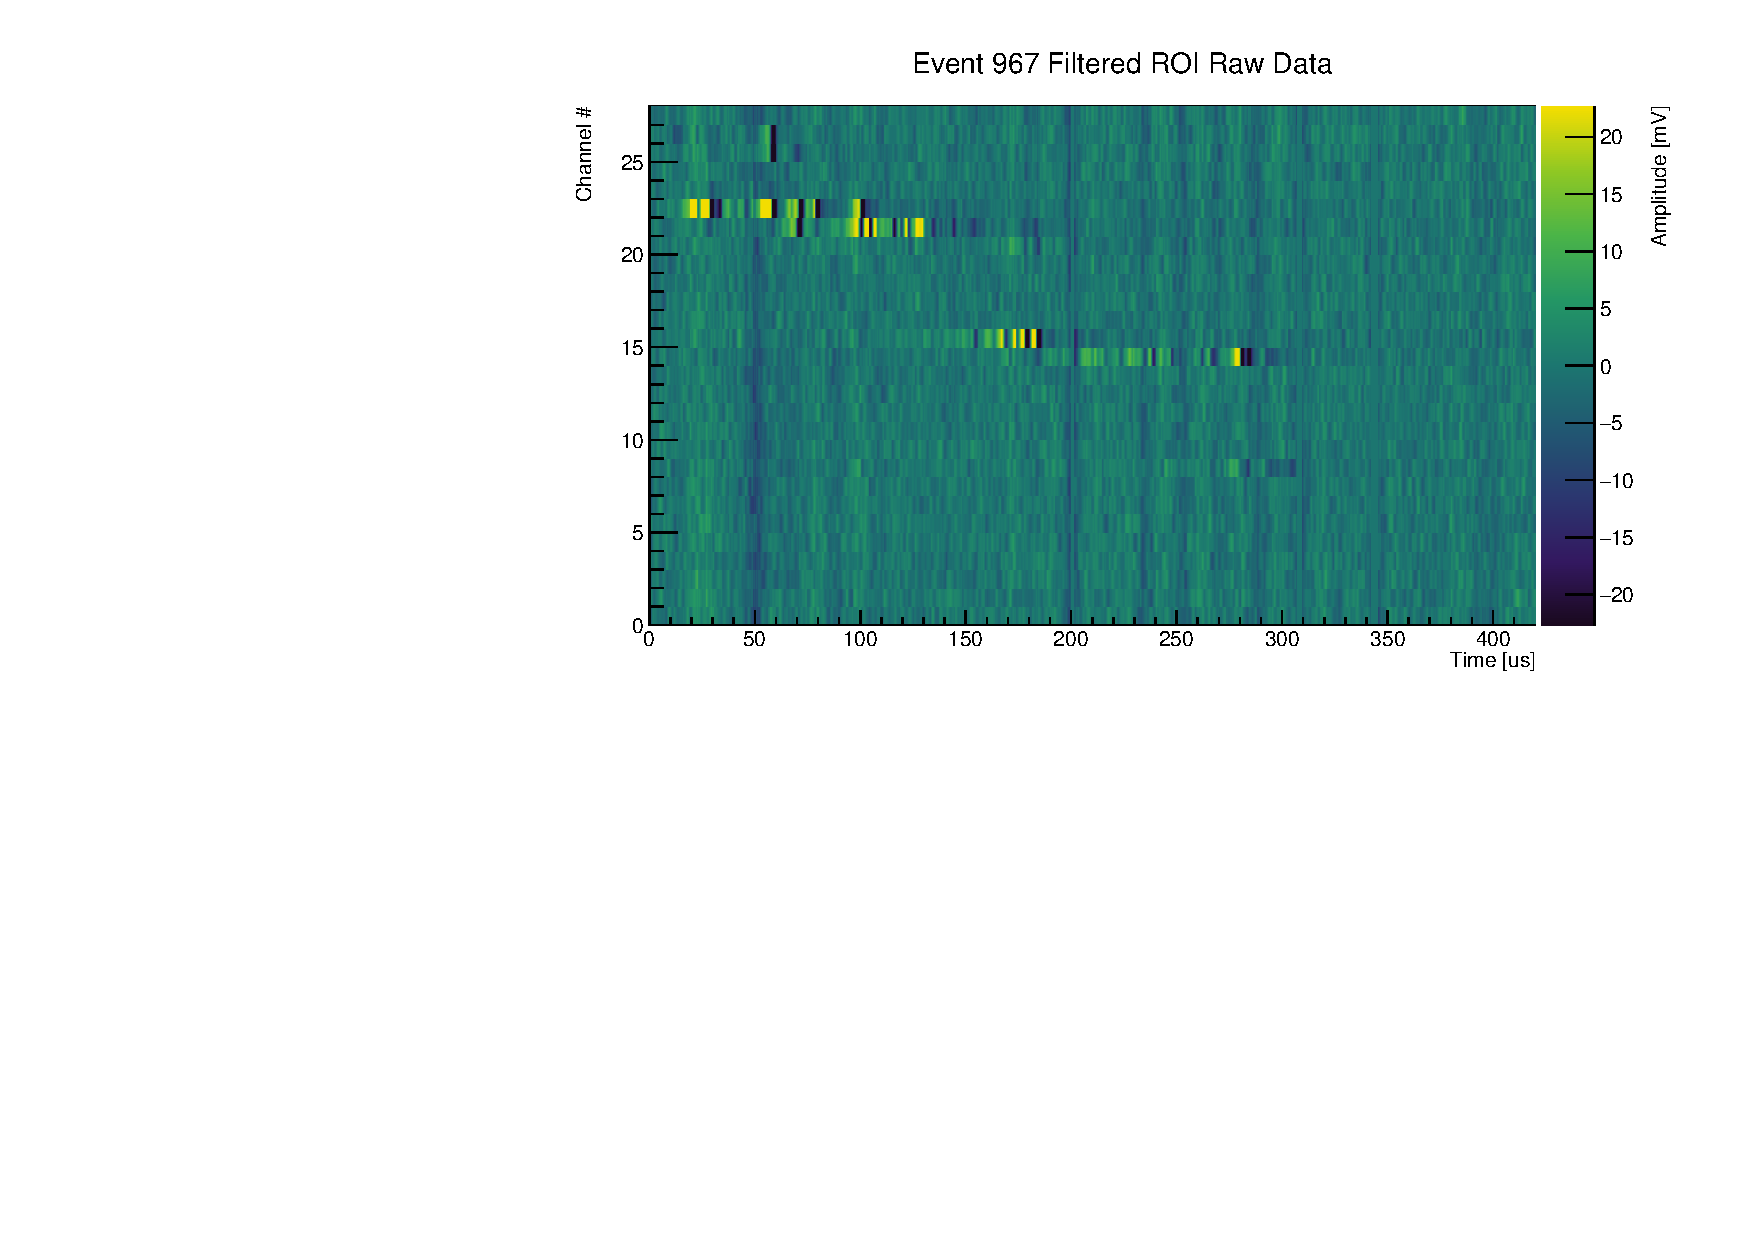
\includegraphics[viewport=0 0 550 290, clip, width=\textwidth]{event967_rawFilteredROI}
		\caption{ROI raw data}
		\label{fig:filteredRawData_b}
	\end{subfigure}
	\caption{Filtered data of a typical MIP event (the same event as in Figures~\ref{fig:unfilteredRawData}, and~\ref{fig:hitFinder} through~\ref{fig:kalman}).
		Note that the colour scale was adjusted to highlight the charge signals (same scale as in Figure~\ref{fig:unfilteredRawData}).
		Therefore, most signal peaks are above/below the maximum/minimum of the colour scale.
		The full range of a typical signal can be seen in Figure~\ref{fig:hitFinder}.}
	\label{fig:filteredRawData}
\end{figure}

The second step applies a recursive pulse finding algorithm (pulse finder).
The following is performed for each channel independently.
Most thresholds employed by the pulse finder are, again, derived from noise levels.
Therefore, noise mean and standard deviation are recalculated after noise filtering.
A peak threshold is defined by multiplying the noise standard deviation by a tunable scaling factor and adding the noise mean.
In the same fashion, an edge threshold lower than the peak threshold is defined to detect the leading and trailing edges of the pulse.
Then, the sample with the highest amplitude is found.
If it is below the peak threshold, the process stops and proceeds to the next channel.
Otherwise, the pulse is scanned in positive and negative directions until it crosses the edge threshold.
After this, the whole pulse is stored and deleted from the input data; then the process starts over with finding the new maximum sample and checking it against the peak threshold.
For stability reasons, the peak threshold derived from the noise levels is compared against an absolute threshold and the higher of the two is applied.
The search is extended to the negative half-pulse for the bipolar ROI pulses, including detection of zero crossing defined by the noise mean.
The different thresholds employed and samples found by this process are illustrated in Figure~\ref{fig:hitFinder}.

\begin{figure}[htb]
	\centering
	\begin{subfigure}{\textwidth}
		\centering
		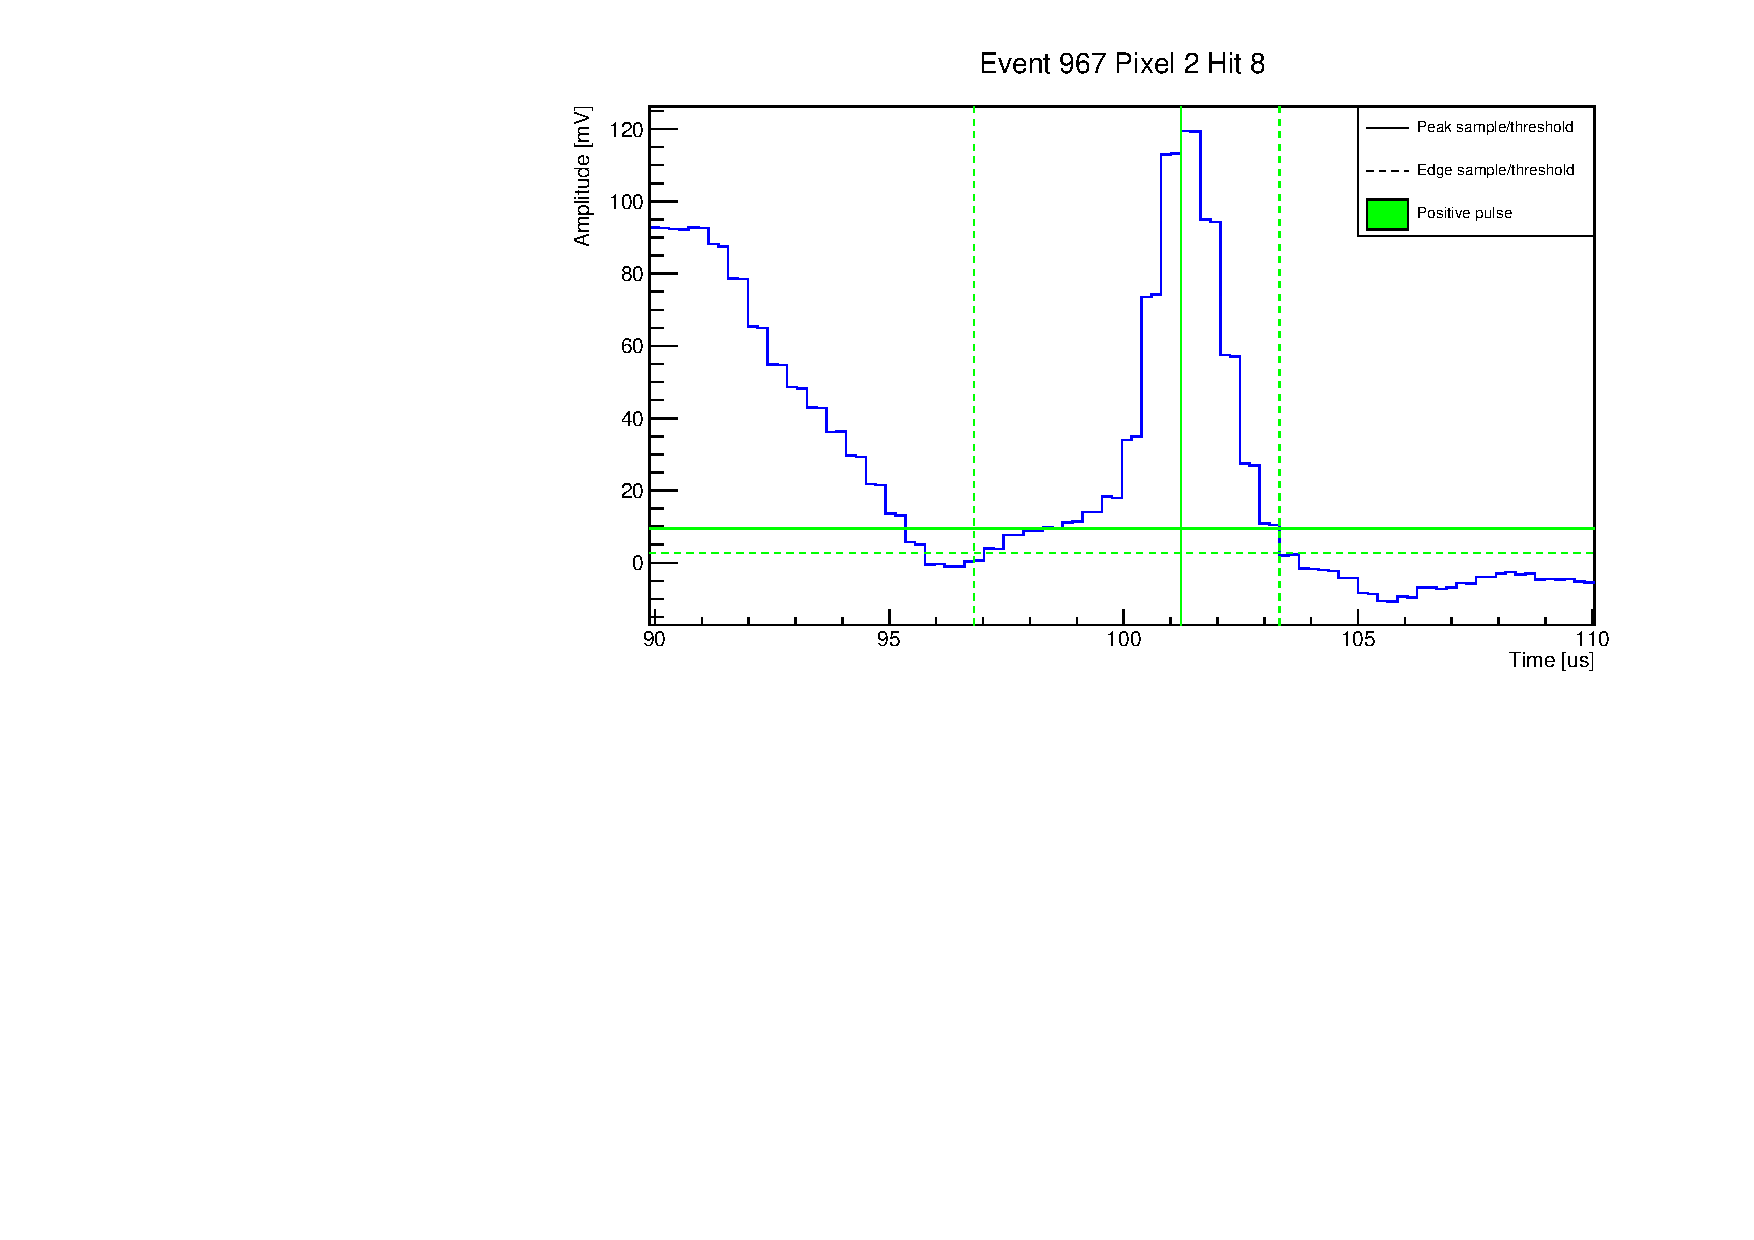
\includegraphics[viewport=0 0 550 290, clip, width=\textwidth, page=1]{event967_pixel2_hit8}\\
		\caption{Pixel pulse\\.}
		\label{fig:hitFinder_a}
	\end{subfigure}
	\begin{subfigure}{\textwidth}
		\centering
		\includegraphics[viewport=0 0 550 290, clip, width=\textwidth, page=3]{event967_pixel2_hit8}
		\caption{ROI pulse}
		\label{fig:hitFinder_b}
	\end{subfigure}
	\caption{Pulse shapes of a single hit of a typical MIP event (the same event as in Figures~\ref{fig:unfilteredRawData},~\ref{fig:filteredRawData},~\ref{fig:pca}, and~\ref{fig:kalman}).
		Superimposed are the thresholds of the pulse finding algorithm.
		Horizontal lines represent thresholds: solid are the minimum thresholds required to be crossed for a pulse to be detected, and dashed are the thresholds used to detect the pulse edges.
		Vertical lines represent the corresponding detected peak/edge samples.
		Colour indicates a positive (green) or negative (red) pulse, or a zero crossing (yellow).
		Note that the yellow zero-crossing threshold is not exactly zero as it is defined by the mean of the noise.}
	\label{fig:hitFinder}
\end{figure}

Identified pulses are then combined into 3D hits by matching every pixel pulse to any ROI pulses overlapping in time.
In Figure~\ref{fig:hitFinder}, a pixel and ROI pulse are matched if their time slices, defined by the vertical dashed lines, overlap.
If a pixel pulse is matched to multiple ROI pulses, an ambiguity occurs, i.e. multiple 3D hit candidates.
The employed 3D hit finding results in a rather high amount of ambiguities, but minimises the number of missed hits.

To resolve the ambiguities, a Principal Component Analysis (PCA) is applied to the 3D hit candidates in a fourth step.
This technique is well established and described in literature, e.g.~\cite{pca}.
The basic idea is to calculate three orthogonal eigenvectors of the 3D space point cloud, representing the three axes of an ellipsoid fitted to the data points.
In case the points form a track, one of these eigenvectors will have a much higher eigenvalue than the other two.
This eigenvector is taken as an estimate for the track direction.
We resolve the ambiguities by selecting the hit candidate closest to the track estimate.
Furthermore, this procedure can be used to recursively reject outliers by forming a cylinder around the track estimate with a radius proportional to the second largest eigenvalue.
All hits outside this cylinder are rejected.
To reject further outliers the PCA is rerun on the remaining points up to three times, or until either no new outliers are rejected, or \SI{40}{\percent} of the hit candidates have been rejected.
In a later stage of reconstructing more complex events, this algorithm can potentially be used to cluster 3D hits in order to separate multiple tracks.
The PCA ambiguity rejection is illustrated in Figure~\ref{fig:pca}.
It should be noted that this step will not be required if the ROI-multiplexing scheme can be avoided, e.g. using cold electronics capable of digitising every single pixel in situ. 

\begin{figure}[htb]
	\centering
	\begin{subfigure}{\textwidth}
		\centering
		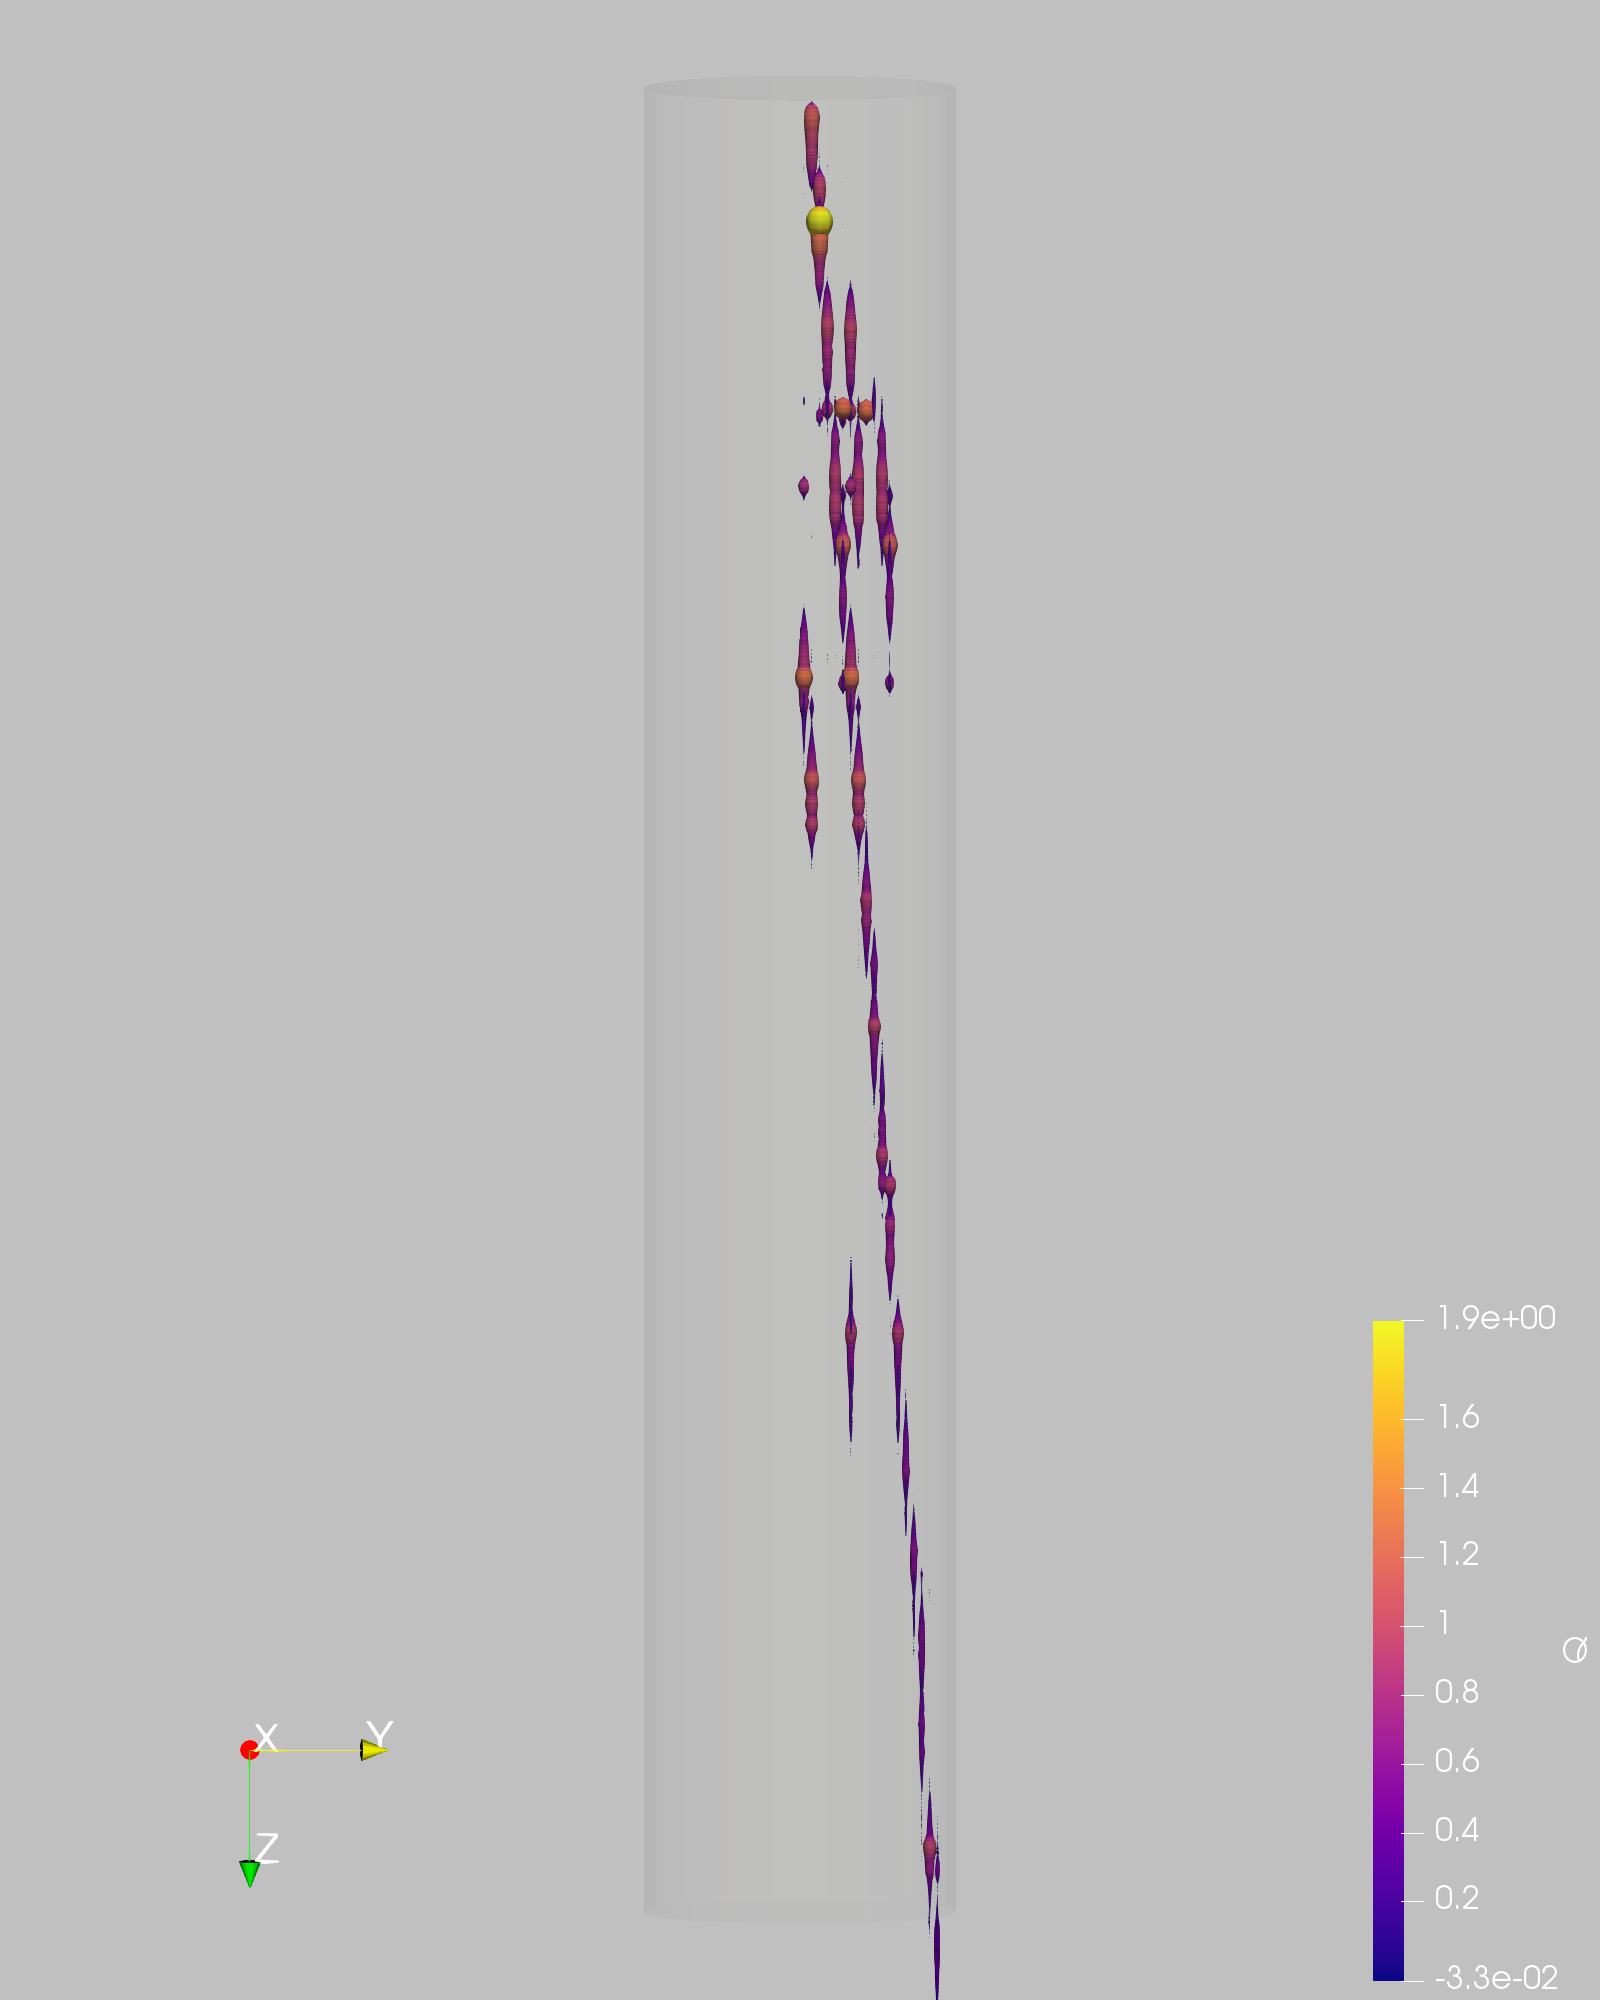
\includegraphics[viewport=600 0 1000 2000, clip, height=\textwidth, angle=90]{event967_pulses_q}
		\caption{Colour-coded amount of collected charge\\.}
		\label{fig:pca_a}
	\end{subfigure}
	\begin{subfigure}{\textwidth}
		\centering
		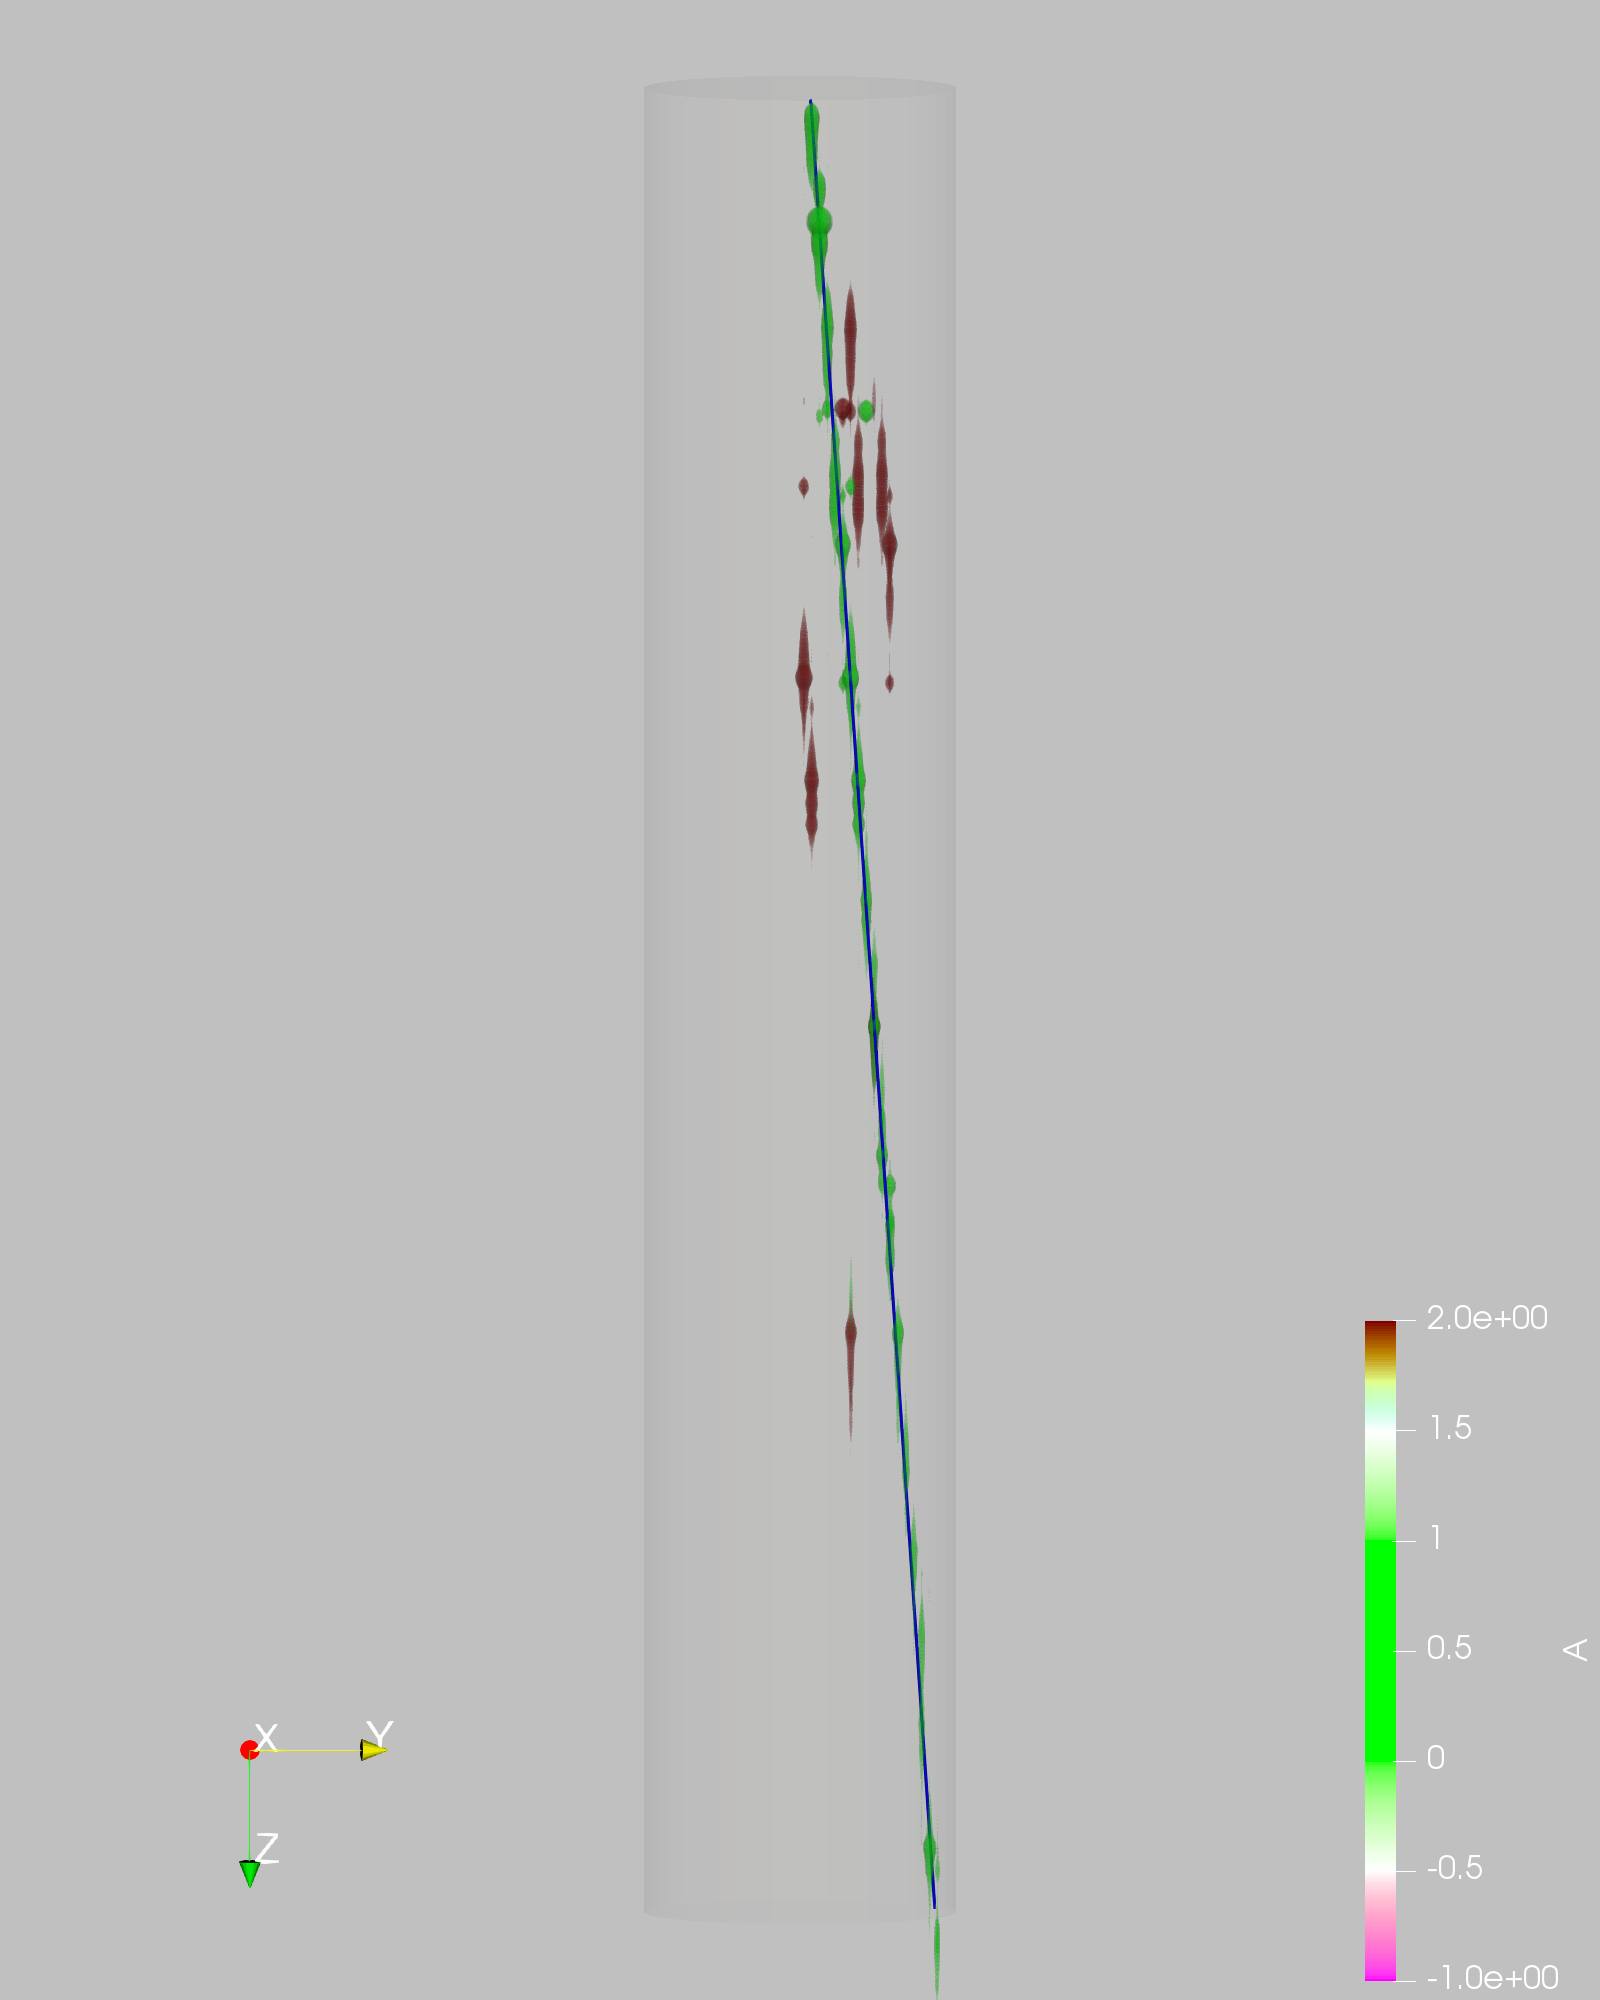
\includegraphics[viewport=600 0 1000 2000, clip, height=\textwidth, angle=90]{event967_pulses_a_pca}
		\caption{Ambiguity resolution employing a principal component analysis:
			Green hits are accepted while dark red ones are rejected.
			This is achieved by selecting the ambiguity closest to the eigenvector of the point cloud with the largest eigenvalue, represented by the blue line.\\.}
		\label{fig:pca_b}
	\end{subfigure}
	\begin{subfigure}{\textwidth}
		\centering
		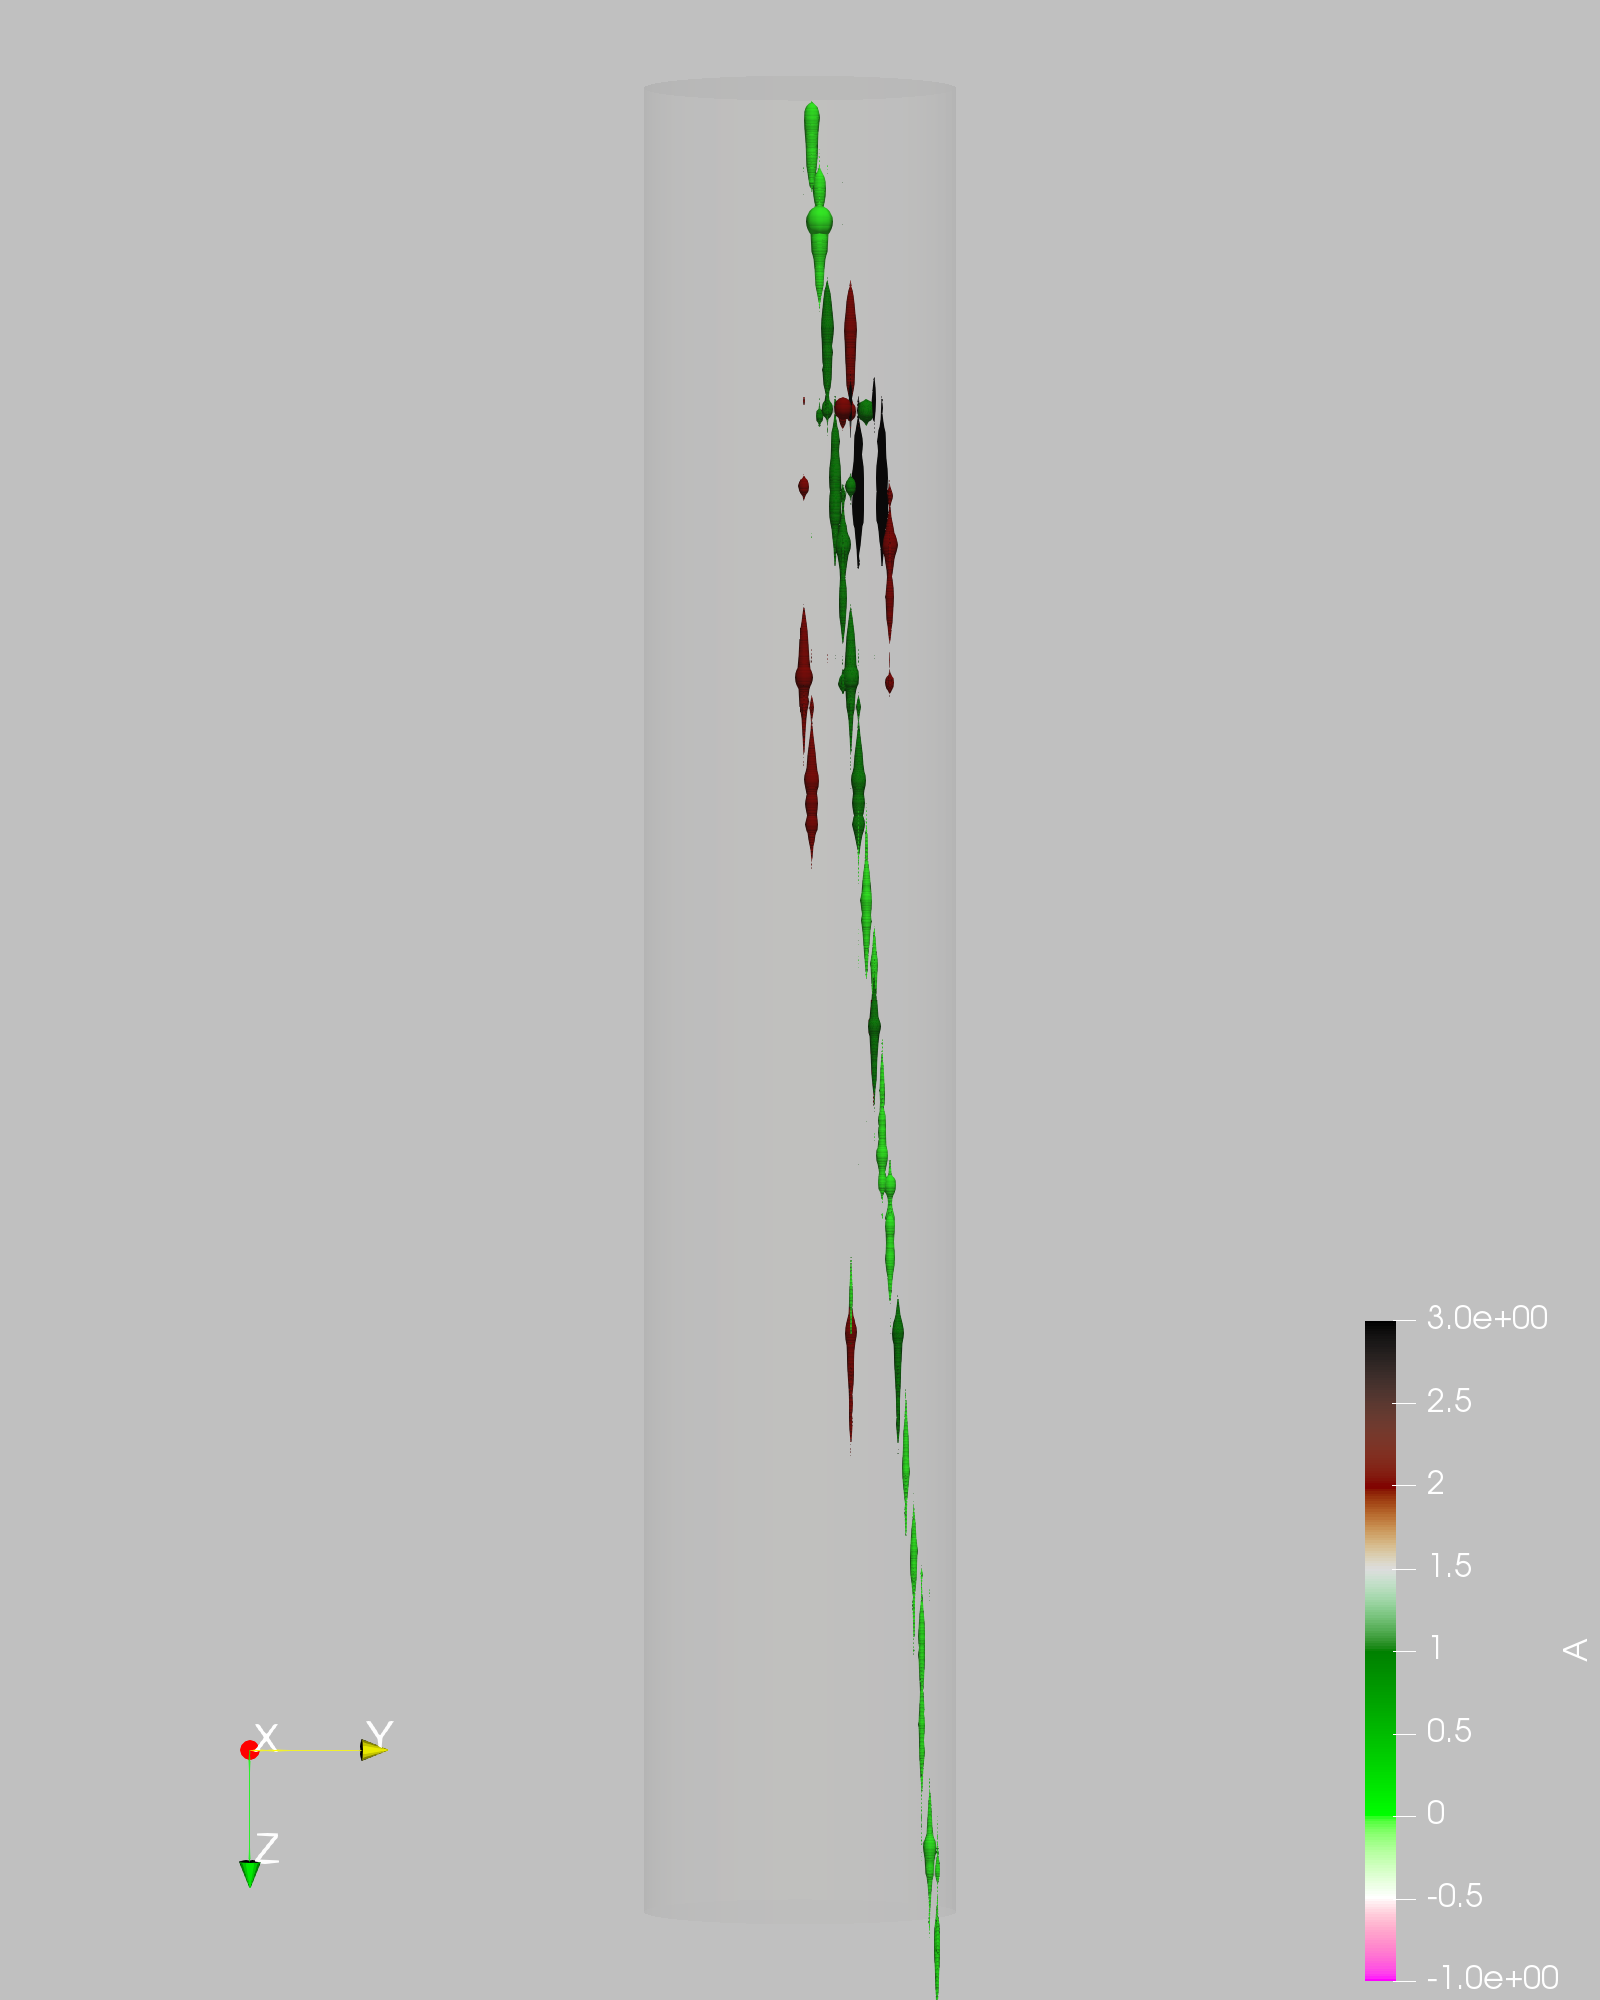
\includegraphics[viewport=600 0 1000 2000, clip, height=\textwidth, angle=90]{event967_pulses_a_det}
		\caption{Colour-coded degree of ambiguity:
			Light green are unambiguous hits while dark green are selected solutions of ambiguous hits.
			Dark red through black are rejected solutions of ambiguous hits where darker colour represents a higher degree of ambiguity.
			As this is a quite clean track with only few short $\delta$ rays, there are no outliers rejected other than the multiplexing ambiguities.}
		\label{fig:pca_c}
	\end{subfigure}
	\caption{Reconstructed 3D hits from the hit finder.
		Axes are the same as in Figure~\ref{fig:kalman}.
		The passing particle is most likely a cosmic $\mu$ entering from the left (the same event as in Figures~\ref{fig:unfilteredRawData} through~\ref{fig:hitFinder}, and~\ref{fig:kalman}).
		Drift direction is from right to left.
		The shapes of the hits encode the shapes of the corresponding pixel pulses.
		Each signal sample is represented by a sphere with its radius proportional to the signal amplitude, resulting in a drop shape.}
	\label{fig:pca}
\end{figure}

The final step consists of a Kalman filter for track identification.
For this, we used the well-established GENFIT track fitting package~\cite{genfit1, genfit2, genfit3}.
Initially we assume a state vector of a minimum-ionising muon with a momentum of \SI{260}{\mega\electronvolt} in the direction of the track estimate from the PCA in the previous step.
The sign of the momentum is chosen such that the muon travels from the atmosphere towards Earth.
Likewise, the fit is started from the 3D hit closest to the atmosphere.
GENFIT then extrapolates the state vector towards the next 3D hit in direction Earth, taking into account ionisation and multiple Coulomb scattering in liquid argon.
The new state vector is improved based on the residuals between the extrapolation and the measured 3D hit.
Finally, the process is repeated by extrapolating the new state vector towards the next 3D hit.
A full track estimate is available after reaching the last 3D hit.
However, the track estimate can still be biased in case of an inferior initial guess.
Therefore, the final state vector is propagated back in space time once again to improve the track estimate.
To improve the estimate even further, the entire process is repeated until the track estimate converges (or a maximum number of iterations is reached).

As a proof of concept we assumed a minimum-ionising muon.
However, the Kalman filter technique is generally applicable to any particle type.
To deal with potential outliers still remaining after the PCA, we chose a recursive algorithm, a so-called \emph{deterministic annealing filter}.
It works by assigning successively lower weights to outliers with each recursion step.
For more details we refer to the respective publications~\cite{genfit1, genfit2, genfit3}.
The resulting track is shown in Figure~\ref{fig:kalman}.

\begin{figure}[htb]
	\centering
	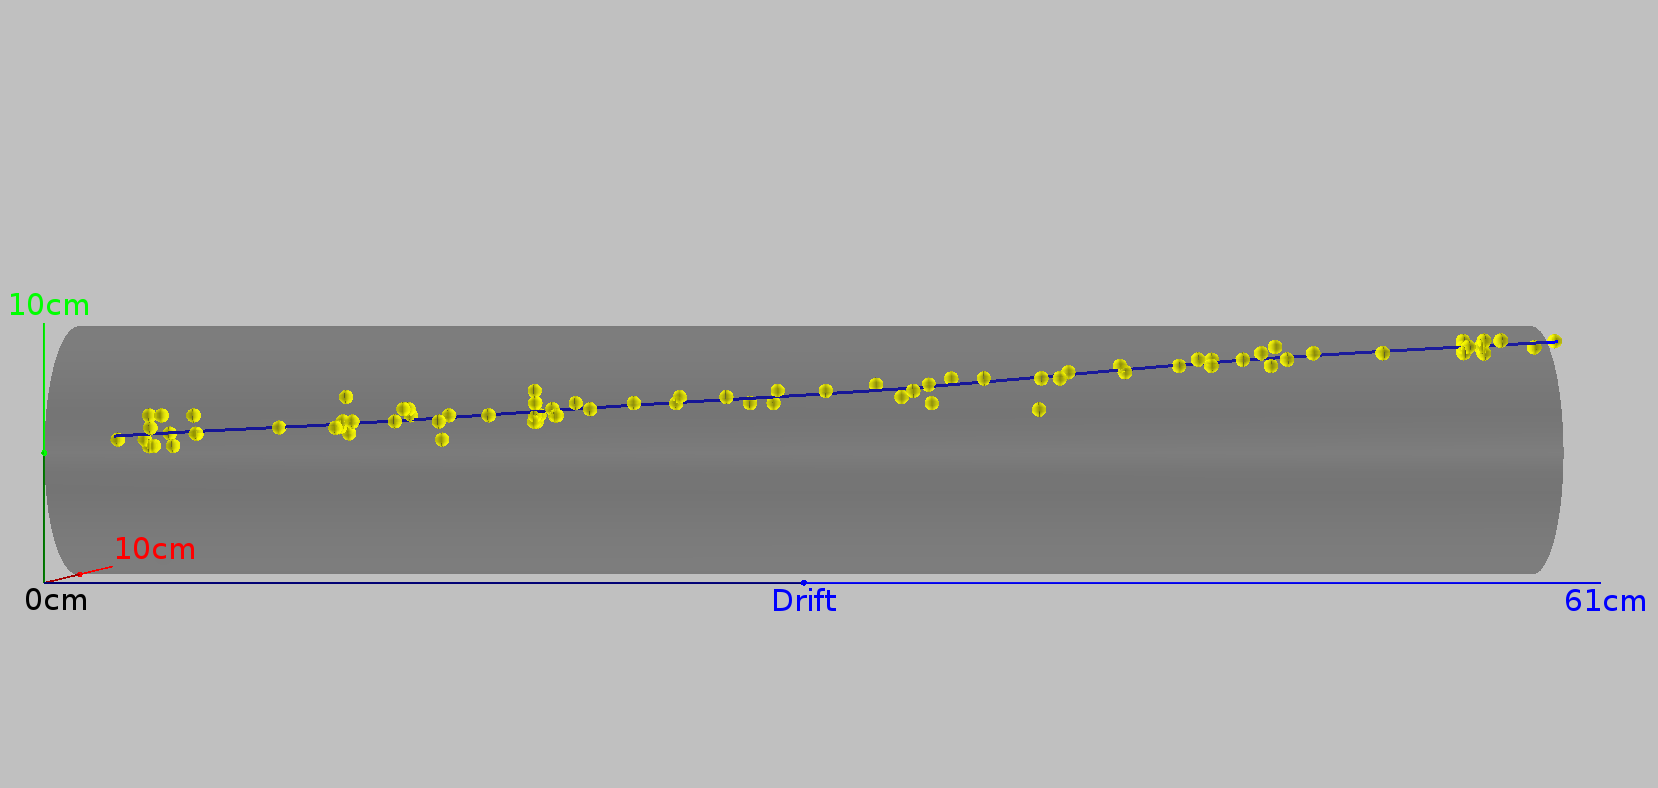
\includegraphics[width=\textwidth]{event967_kalman}
	\caption{Track fitted by the Kalman filter.
		The TPC volume is shown in faint grey.
		The passing particle is most likely a cosmic $\mu$ entering from the left (the same event as in Figures~\ref{fig:unfilteredRawData} through~\ref{fig:pca}).
		Drift direction is from right to left.
		The yellow points are the input to the Kalman filter, the accepted 3D hits from the principal components analysis.
		Blue is the output, a fitted track taking into account ionisation losses and multiple scattering in LAr.}
	\label{fig:kalman}
\end{figure}

\afterpage{\clearpage}

In the near future, the Kalman filter will be capable of fitting the particle momentum and/or even particle type to the data.
However, at the time of this writing, this was not implemented.
In particular, the momentum stays roughly at the initial guess of \SI{260}{\mega\electronvolt}.
A potential explanation for this is that the resolution of our detector is too low to estimate momentum from multiple scattering.
Another explanation might be the hit finder missing hits due to non-optimal tuning.
Proper tuning of the reconstruction requires a full simulation chain of the detector which is not yet available.
Using data to tune the reconstruction is prone to the introduction of circular biases.
On the other hand, most of the difficulties emerge from the multiplexing ambiguities and their resolution.
While the presented 3D readout already reduces the reconstruction complexity compared to a classical wire readout, an ambiguity-free readout will make reconstruction even easier by completely eliminating the need to resolve ambiguities.

\clearpage


\section{Conclusions} \label{sec:Summary}

We have presented a proof of concept for a pixelated charge readout for single-phase LArTPCs by successfully building and operating a pixelated LArTPC, and reconstructed 3D tracks of cosmic muons crossing the TPC.
The requirement of high readout channel number has not yet been addressed.
In this first implementation, we have used existing wire readout electronics in conjunction with analogue multiplexing which introduces ambiguities.
Although much improved compared to classical wire readouts, the signal to noise ratio of and the multiplexing ambiguities complicated reconstruction.
This work shows that it is of paramount importance to be capable of digitising the charge signals at cryogenic temperatures allowing for digital multiplexing and thus enabling a true, ambiguity-free, 3D LArTPC charge readout.
Work is currently under way to develop bespoke pixel readout electronics, based on the requirements highlighted by this demonstration. 
Once this last remaining problem is solved, pixelated charge readouts will enable the true 3D tracking capabilities of single-phase LArTPCs.
This work has been a success in reconstructing the first particle track in a LArTPC using a pixelated charge readout.   
This technology will provide the necessary reconstruction efficiency and background rejection to enable LArTPCs to operate in high-multiplicity environments, such as the DUNE near detector.


%%%%%%%%%%%%%%%%%%%%%%%%%%%%%%%%%%%%%%%%%%
\vspace{6pt} 

%%%%%%%%%%%%%%%%%%%%%%%%%%%%%%%%%%%%%%%%%%
%% optional
%\supplementary{The following are available online at \linksupplementary{s1}, Figure S1: title, Table S1: title, Video S1: title.}

% Only for the journal Methods and Protocols:
% If you wish to submit a video article, please do so with any other supplementary material.
% \supplementary{The following are available at \linksupplementary{s1}, Figure S1: title, Table S1: title, Video S1: title. A supporting video article is available at doi: link.}

%%%%%%%%%%%%%%%%%%%%%%%%%%%%%%%%%%%%%%%%%%
\authorcontributions{Conceptualization, J.A., F.S., M.W., D.L., M.L., C.U.B.R.V.R, M.A., A.E., I.K, D.G., J.S.; Funding acquisition, A.E., I.K., M.W.; Investigation, U.K., F.S., M.W., D.L., M.L., C.B.U.R.V.R, M.A., A.E., I.K, D.G., J.S. All authors have read and agreed to the published version of the manuscript. }

%%%%%%%%%%%%%%%%%%%%%%%%%%%%%%%%%%%%%%%%%%
\funding{
\textls[-5]{This research was funded by the Swiss National Science Foundation and the Canton of Bern, Switzerland}.
%Please add: ``This research received no external funding'' or ``This research was funded by NAME OF FUNDER grant number XXX.'' and  and ``The APC was funded by XXX''. Check carefully that the details given are accurate and use the standard spelling of funding agency names at \url{https://search.crossref.org/funding}, any errors may affect your future funding.
}

%%%%%%%%%%%%%%%%%%%%%%%%%%%%%%%%%%%%%%%%%%
\acknowledgments{The authors would like to thank Yun-Tse Tsai and Tracy L. Usher of SLAC National Accelerator Laboratory, California, USA, for their valuable advice and guidance in the development of the 3D event reconstruction. 
The authors would like to thank Dean Shooltz of Michigan State University, Michigan, USA, for his extensive help in the design of the differential amplifiers..}

%%%%%%%%%%%%%%%%%%%%%%%%%%%%%%%%%%%%%%%%%%
\conflictsofinterest{
The authors declare no conflict of interest.
The funders had no role in the design of the study; in the collection, analyses, or interpretation of data; in the writing of the manuscript, or in the decision to publish the results
%Declare conflicts of interest or state ``The authors declare no conflict of interest.'' Authors must identify and declare any personal circumstances or interest that may be perceived as inappropriately influencing the representation or interpretation of reported research results. Any role of the funders in the design of the study; in the collection, analyses or interpretation of data; in the writing of the manuscript, or in the decision to publish the results must be declared in this section. If there is no role, please state ``The funders had no role in the design of the study; in the collection, analyses, or interpretation of data; in the writing of the manuscript, or in the decision to publish the results''.
}

%%%%%%%%%%%%%%%%%%%%%%%%%%%%%%%%%%%%%%%%%%
\reftitle{References}

% Please provide either the correct journal abbreviation (e.g. according to the “List of Title Word Abbreviations” http://www.issn.org/services/online-services/access-to-the-ltwa/) or the full name of the journal.
% Citations and References in Supplementary files are permitted provided that they also appear in the reference list here. 

%=====================================
% References, variant A: external bibliography
%=====================================
%\externalbibliography{yes}
\bibliography{MDPI_Pixel.bib}
\bibliographystyle{mdpi.bst}

% The following MDPI journals use author-date citation: Arts, Econometrics, Economies, Genealogy, Humanities, IJFS, JRFM, Laws, Religions, Risks, Social Sciences. For those journals, please follow the formatting guidelines on http://www.mdpi.com/authors/references
% To cite two works by the same author: \citeauthor{ref-journal-1a} (\citeyear{ref-journal-1a}, \citeyear{ref-journal-1b}). This produces: Whittaker (1967, 1975)
% To cite two works by the same author with specific pages: \citeauthor{ref-journal-3a} (\citeyear{ref-journal-3a}, p. 328; \citeyear{ref-journal-3b}, p.475). This produces: Wong (1999, p. 328; 2000, p. 475)


%%%%%%%%%%%%%%%%%%%%%%%%%%%%%%%%%%%%%%%%%%

%% for journal Sci
%\reviewreports{\\
%Reviewer 1 comments and authors’ response\\
%Reviewer 2 comments and authors’ response\\
%Reviewer 3 comments and authors’ response
%}

%%%%%%%%%%%%%%%%%%%%%%%%%%%%%%%%%%%%%%%%%%
\end{document}

